%% Glaukopis -- journal manuscript, v1.6 (2026-10-24).
%% Built from doc/v1.5 (Computers & Security)/glaukopis_cs_v1.5.tex in
%% response to the Computers & Security reviews (COSE-D-26-05507, two
%% reviewers, 17 and 22 October 2026). RESPONSE_TO_REVIEWERS_v1.6.md in this
%% folder maps every review comment to the change made. New numbers in this
%% version (CSE-shard output profile, VSP metric-level accuracy and error
%% direction, single-stage reference run, MMLU-Pro subject deltas) are
%% produced by analysis/v16_additions.py from the same artifacts as v1.5.
%% Compile: bash build.sh   (pdflatex -> bibtex -> pdflatex x2)
%% The \journal{} line below is a placeholder; set it to the target venue.
\documentclass[preprint,12pt,authoryear]{elsarticle}
\usepackage[T1]{fontenc}
\usepackage{lmodern}
\usepackage{amsmath,amssymb}
\usepackage{booktabs,array,tabularx,multirow}
\usepackage{graphicx}
\usepackage{xcolor}
\usepackage{xurl}
\usepackage{tikz}
\usetikzlibrary{arrows.meta,positioning,fit,backgrounds,calc}
\usepackage{pgfplots}
\usepgfplotslibrary{groupplots}
%% compat=1.15 is the highest level accepted by the pgfplots 1.15 (2017) that
%% TexpadTeX/Texifier bundles; newer pgfplots (TeX Live ships 1.18.1) accepts it
%% too, so both toolchains render this figure identically. Do not raise it
%% without checking the version available in every build environment used.
\pgfplotsset{compat=1.15}
\usepackage{listings}
\usepackage{lineno}
\usepackage[hidelinks]{hyperref}
\modulolinenumbers[5]
\setlength{\emergencystretch}{2em}
\renewcommand{\topfraction}{0.95}
\renewcommand{\bottomfraction}{0.95}
\renewcommand{\textfraction}{0.03}
\renewcommand{\floatpagefraction}{0.75}
\setcounter{topnumber}{4}\setcounter{bottomnumber}{4}\setcounter{totalnumber}{8}
\lstset{basicstyle=\footnotesize\ttfamily,breaklines=true,columns=fullflexible,keepspaces=true,frame=single,showstringspaces=false}
\newcommand{\code}[1]{\path{#1}}
\newsavebox{\fitbox}
\newcommand{\fitwidth}[1]{\sbox{\fitbox}{#1}\ifdim\wd\fitbox>\textwidth\resizebox{\textwidth}{!}{\usebox{\fitbox}}\else\usebox{\fitbox}\fi}
\newcommand{\ci}[2]{{\scriptsize[#1,\,#2]}}
\newcommand{\Abal}{A_{\mathrm{bal}}}
\newcommand{\Bbal}{B_{\mathrm{bal}}}
\newcommand{\Tbal}{T_{\mathrm{bal}}}
\definecolor{seriesblue}{HTML}{2A78D6}
\definecolor{refgray}{HTML}{52514E}
%% ---------------------------------------------------------------------------
%% Compatibility shim for elsarticle < 3.0. \affiliation and the highlights
%% environment were introduced in elsarticle 3.x (TeX Live ships 3.3,
%% 2020/11/20). Older classes, such as the 1.2.0 (2009) copy bundled with
%% TexpadTeX/Texifier, leave both undefined, so their arguments are typeset
%% as raw text on a spurious first page and the affiliation labels never
%% resolve. When the class already defines them this block does nothing.
\makeatletter
\@ifundefined{affiliation}{%
  \RequirePackage{keyval}%
  \def\els@aff@text{}%
  \def\els@aff@add#1{%
    \ifx\els@aff@text\@empty\gdef\els@aff@text{#1}%
    \else\g@addto@macro\els@aff@text{, #1}\fi}%
  \define@key{els@aff}{organization}{\els@aff@add{#1}}%
  \define@key{els@aff}{addressline}{\els@aff@add{#1}}%
  \define@key{els@aff}{city}{\els@aff@add{#1}}%
  \define@key{els@aff}{postcode}{\els@aff@add{#1}}%
  \define@key{els@aff}{state}{\els@aff@add{#1}}%
  \define@key{els@aff}{country}{\els@aff@add{#1}}%
  \newcommand{\affiliation}[2][]{%
    \gdef\els@aff@text{}%
    \setkeys{els@aff}{#2}%
    \if\relax\detokenize{#1}\relax
      \edef\els@aff@tmp{\noexpand\address{\unexpanded\expandafter{\els@aff@text}}}%
    \else
      \edef\els@aff@tmp{\noexpand\address[#1]{\unexpanded\expandafter{\els@aff@text}}}%
    \fi
    \els@aff@tmp}%
}{}
\@ifundefined{highlights}{%
  \newbox\els@hlbox
  \def\els@prelimauthors{}%
  \let\els@author@orig\author
  \def\author{\@ifnextchar[{\els@author@opt}{\els@author@noopt}}%
  \def\els@author@opt[#1]#2{\els@prelimauthor{#2}\els@author@orig[#1]{#2}}%
  \def\els@author@noopt#1{\els@prelimauthor{#1}\els@author@orig{#1}}%
  \def\els@prelimauthor#1{\g@addto@macro\els@prelimauthors{\els@prelimsep#1}}%
  \newenvironment{highlights}{%
    \global\setbox\els@hlbox=\vbox\bgroup\hsize=\textwidth\def\baselinestretch{1}%
    \noindent{\Large Highlights}\par\vskip12pt
    \noindent\textbf{\@title}\par\vskip6pt
    \noindent{\let\corref\@gobble\let\fnref\@gobble\let\tnoteref\@gobble
      \def\els@prelimsep{\def\els@prelimsep{, }}\els@prelimauthors}\par\medskip
    \begin{itemize}}{\end{itemize}\egroup}%
  \let\els@maketitle@orig\maketitle
  \def\maketitle{%
    \ifvoid\els@hlbox\else
      \thispagestyle{empty}\unvbox\els@hlbox\clearpage\setcounter{page}{1}%
    \fi
    \els@maketitle@orig}%
}{}
\makeatother
%% ---------------------------------------------------------------------------
\journal{Journal of Information Security and Applications}  %% placeholder: set to the venue chosen for submission

\begin{document}
\begin{frontmatter}

\title{Glaukopis: Auditable Graph-Grounded Instruction Tuning for Cyber Threat Intelligence}

\author[fau,asg]{Peter J. Worth Jr.\corref{cor1}}
\ead{pworthjr@athenasecuritygrp.com}
\author[fau,asg]{Ionut Cardei}
\author[rai]{Salman Ahmad}
\author[rai]{Muhammad Mamoon Khan}
\cortext[cor1]{Corresponding author. ORCID: 0000-0003-4211-3866.}
\affiliation[fau]{organization={Department of Electrical Engineering and Computer Science, Florida Atlantic University},city={Boca Raton},state={FL},country={USA}}
\affiliation[asg]{organization={Athena Security Group, LLC},country={USA}}
%% TODO (authors): confirm the legal entity name used for the affiliation, funding and competing-interest statements (Athena Security Group is the trade name; the legal entity may be Athena Software Group, Inc.). Use one form consistently, including in the glaukopis2026software bib entry.
\affiliation[rai]{organization={RevolveAI}}
%% TODO (authors): confirm the RevolveAI city/country and each author's ORCID before submission.

\begin{abstract}
Security operations centers increasingly use language models for cyber threat intelligence (CTI) work: mapping a vulnerability to its weakness class, extracting the ATT\&CK technique behind an observed behavior, recommending mitigations, or attributing an intrusion to a known actor. Organizations that must serve such a model locally need to specialize an open-weight model, know where its training data came from, and know what the specialization cost in other capabilities. Glaukopis addresses all three. It constructs instruction-tuning data by executing typed queries over Ariadne, a knowledge graph integrating twelve public CTI sources, so that every training target is traceable to the graph facts that produced it, and it fine-tunes Qwen2.5-32B-Instruct in four stages while retaining each stage's checkpoint, so that gains and losses can be located rather than inferred from one final score. Evaluation uses three CTI benchmarks, a general-reasoning diagnostic (MMLU-Pro), six hosted frontier models and a security-specialized open model as references, item-level bootstrap intervals, and error taxonomies. The final checkpoint raises the three-benchmark mean from 57.7 to 65.0; attack-technique extraction improves from 18.2 to 65.8 and mitigation scoring from 7.6 to 62.5. The gains are confined to the benchmark whose schemas the training data targets; two benchmarks built by other groups are unchanged, and MMLU-Pro falls by 11.6 points. Checkpoint-level analysis locates the cost: one stage of 17,320 short structured-answer drills collapses actor attribution and shifts severity judgments toward network-reachable, unauthenticated profiles. A single-stage run performs comparably on the aligned benchmark, so no advantage is claimed for the schedule. The contribution is a traceable data-construction method and a diagnostic protocol that shows what specialization gives and takes away.
\end{abstract}

%% Highlights are uploaded to Elsevier as a separate file (highlights.txt in this
%% folder), so the environment below stays commented out: with elsarticle 3.x it
%% would typeset an extra unnumbered Highlights page before the title page.
%% Re-enable it only if a Highlights page inside the manuscript PDF is wanted.
%\begin{highlights}
%\item Sophia materializes CTI instruction targets by executing typed graph queries
%\item Retained checkpoints expose task interference hidden by a single final score
%\item Balanced attribution aggregation: 65.0 vs.\ 57.7 base, all gain in aligned tasks
%\item Item-level audit: attribution collapse is semantic, not a parsing artifact
%\item Gold-fact overlap, n-gram screening and cost accounting are quantified
%\end{highlights}

\begin{keyword}
cyber threat intelligence \sep instruction fine-tuning \sep knowledge graphs \sep data provenance \sep language-model evaluation \sep catastrophic interference
\end{keyword}

\end{frontmatter}

\linenumbers

\section{Introduction}\label{sec:intro}
Cyber threat intelligence (CTI) is the practice of collecting, structuring, and acting on knowledge about adversaries, their techniques, and the vulnerabilities they exploit. Much of that knowledge is published as public catalogs with stable identifiers: the MITRE ATT\&CK matrix of adversary techniques (T-codes) and groups (G-codes), the Common Weakness Enumeration (CWE), the Common Vulnerabilities and Exposures list (CVE) with its CVSS severity vectors, and detection and mitigation catalogs built around them. A security analyst's routine work consists largely of mapping between these catalogs under time pressure: deciding which weakness class explains a new vulnerability description, which ATT\&CK technique an observed behavior corresponds to, which mitigations apply to a technique, and which known actor an intrusion resembles. These are exactly the tasks that recent CTI benchmarks such as CTIBench and AthenaBench measure, because a general language model can be fluent and still return a parent technique instead of the requested sub-technique, a related but wrong CWE, or a malformed structured answer \citep{alam2024ctibench,alam2025athenabench}.

Many security operations centers (SOCs) would like to use a language model for this work but cannot send incident data to a hosted service because of contractual, confidentiality, or data-residency constraints. The practical option is to take an open-weight model, specialize it on CTI data, and serve it locally. That raises two questions that this article addresses. The first is about the training data: when instruction-tuning examples are synthesized (by a model, by annotators, or by templates), can a reviewer trace a given training target back to the public fact that justifies it? The second is about the specialization itself: a single aggregate score for the final model does not say which capabilities improved, which regressed, and at which point in training the regression occurred.

Glaukopis is the framework we built to answer both questions; its components are named after figures from Greek mythology and are introduced here once. \emph{Ariadne} is a knowledge graph, stored in Neo4j, that integrates twelve public CTI sources (Section~\ref{sec:data}). \emph{Sophia} is a template engine that produces an instruction-tuning example by executing a typed query against Ariadne and rendering the returned graph binding into an instruction, an optional context, and a target answer; the target is therefore a deterministic function of specific graph facts, and every CTI example in the corpus carries the identifier of the template that produced it. The training recipe fine-tunes Qwen2.5-32B-Instruct, a 32-billion-parameter open-weight model that fits on two 80-GB GPUs for serving, in four supervised stages, and keeps the checkpoint after each stage. Evaluating every retained checkpoint on the same benchmark suite turns training into a sequence of observable transitions, which is what allows us to locate when a capability is lost and to inspect the responses that lost it.

The evaluation must be read with two facts in mind, both of which bear on independence. First, the training templates deliberately cover the task schemas that the AthenaBench benchmark tests, because those schemas are the operational tasks the model is meant to perform. Second, AthenaBench was created by a team that includes two of the present authors (Worth and Ahmad). The training data and the benchmark items were built by different pipelines from different inputs, and we quantify their overlap at the level of 13-grams, entities, and gold facts (Section~\ref{sec:overlap}). But the people who designed the benchmark also designed the training templates, and that shared knowledge of the task schemas is a form of alignment that no overlap measurement removes. We therefore treat AthenaBench as the aligned, in-domain benchmark and rely on two benchmarks built by unrelated groups (CyberSOCEval and CyberMetric) and on a general-reasoning diagnostic (MMLU-Pro) as the independent evidence. On that evidence the final checkpoint does not improve over the base model, and on MMLU-Pro it loses 11.6 points.

The results should be understood accordingly. Glaukopis demonstrates a traceable way to construct CTI instruction data and a diagnostic protocol that shows what a specialization recipe gives and takes away. It does not demonstrate that a four-stage schedule is better than a single-stage one; a single-stage run from the project's own record performs comparably on the aligned benchmark (Section~\ref{sec:singlestage}), and a matched control has not been trained. The contributions are: (i) a CTI data-construction method in which every training target resolves to an executed graph query over public-source identifiers; (ii) a retained-checkpoint evaluation protocol with item-level uncertainty, response-level error taxonomies, and a mechanistic account of the two regressions observed; (iii) a quantified audit of training--evaluation overlap at the n-gram, entity, and gold-fact levels; and (iv) an evaluation against the base model, a security-specialized open model, six hosted frontier models, and a single-stage run, with explicit statements of what each comparison does and does not control. The software is source-available \citep{glaukopis2026software}.

The rest of the article is organized as follows. Section~\ref{sec:overview} gives a one-page overview of the system and defines the names and acronyms used throughout. Section~\ref{sec:problem} states the problem formally. Section~\ref{sec:related} reviews related work and positions the system. Sections~\ref{sec:data} and~\ref{sec:training} describe the data pipeline and the training recipe, with the rationale for each design choice. Section~\ref{sec:evaluation} describes the benchmarks, baselines, aggregation conventions, overlap audit, and uncertainty estimates. Section~\ref{sec:results} reports and interprets the results, including the mechanisms behind the two regressions. Section~\ref{sec:cost} reports inference efficiency. Section~\ref{sec:limits} discusses threats to validity, and Section~\ref{sec:conclusion} concludes.

\section{System overview and terminology}\label{sec:overview}
Figure~\ref{fig:pipeline} shows the three parts of the system as configured for the release evaluated here (internally, release v21). Public CTI sources are loaded into Ariadne; Sophia executes templates against Ariadne to produce four training shards; the shards are used in four stages of supervised fine-tuning; and every retained checkpoint is evaluated on the same suite. Table~\ref{tab:glossary} defines the names that recur in the article. Two conventions apply throughout. A \emph{shard} is a serialized training file produced by one Sophia run; a \emph{stage} is one fine-tuning pass that consumes one or more shards and starts from the checkpoint of the previous stage. Checkpoints are named after the stage that produced them (Core, +TAA, CSE, Recal-32B), and ``base'' denotes the unmodified Qwen2.5-32B-Instruct model.

\begin{table}[!htbp]
\centering\footnotesize
\caption{Names and acronyms used in this article.}\label{tab:glossary}
\begin{tabularx}{\textwidth}{@{}p{3.2cm}X@{}}
\toprule Term & Meaning \\\midrule
Glaukopis & The framework as a whole: graph, template engine, training recipe, evaluation harness. \\
Ariadne & The Neo4j knowledge graph that integrates twelve public CTI sources (Section~\ref{sec:data}). \\
Sophia & The template engine that executes typed graph queries against Ariadne and renders the bindings into instruction-tuning records. \\
Core-A, Core-B & The two Sophia shards used in Stage 1: Core-A covers broad CTI knowledge and question formats; Core-B covers the four catalog-mapping schemas (mitigation, technique extraction, severity, root cause). \\
TAA shard; +TAA & The shard of threat-actor-attribution drills and the checkpoint after training on it (Stage 2). \\
CSE shard; CSE & The shard of SOC-style multiple-select drills whose answers are letter sets, named after CyberSOCEval, and the checkpoint after training on it (Stage 3). \\
Recal-32B, Recal-14B & Two Stage-4 ``recalibration'' passes over a mixture of earlier shards, trained from the CSE checkpoint with a 32B-tuned and a 14B-derived recipe respectively. Recal-32B is the released checkpoint. \\
AthenaBench & CTI benchmark with six tasks: CKT (CTI knowledge, multiple choice), ATE (attack-technique extraction), RCM (root-cause mapping, CVE$\to$CWE), RMS (risk-mitigation strategy), VSP (vulnerability-severity prediction, CVSS vector), TAA (threat-actor attribution, in a Classic and a Canonical form) \citep{alam2025athenabench}. \\
CyberSOCEval & Benchmark of malware-analysis and threat-intelligence multiple-select questions built by Meta and CrowdStrike \citep{deason2025cybersoceval}. \\
CyberMetric & Cybersecurity multiple-choice benchmark, 2K and 10K tiers \citep{tihanyi2024cybermetric}. \\
MMLU-Pro & General multi-subject reasoning benchmark used as a diagnostic for lost general capability \citep{wang2024mmlupro}. \\
$\Tbal$, $\Abal$, $\Bbal$ & Balanced attribution score, AthenaBench macro-score, and three-benchmark mean (Section~\ref{sec:aggregation}). \\
\bottomrule
\end{tabularx}
\end{table}

\section{Problem formulation and scope}\label{sec:problem}
\subsection{Inputs, outputs, and provenance}
Let $G_t=(V_t,E_t,A_t)$ be a versioned CTI graph at snapshot $t$, comprising typed entities, relationships, and attributes. A template $\tau$ specifies a typed query $q_\tau$, constraints, and rendering functions. For a returned binding $b\in q_\tau(G_t)$, Sophia constructs
\begin{align}
 r_{\tau,b}&=\bigl(i_\tau(b),x_\tau(b),y_\tau(b)\bigr),\\
 y_\tau(b)&=\operatorname{render}_{\tau}\bigl(q_\tau(G_t),b\bigr).
\end{align}
Here $i$ is the instruction, $x$ the optional context or question, and $y$ the supervised target. An audit links the row to its template, graph snapshot, and bound public identifiers. In the released data these provenance elements are carried by the generation artifacts and by a per-row template identifier (\code{shortname}) and source tag; the three-field Alpaca training record alone does not encode a complete immutable provenance manifest.

The resulting model $p_\theta(y\mid i,x)$ is trained with ordinary next-token cross-entropy. For stage $s$ and its training set $D_s$, the objective is
\begin{equation}
 \mathcal{L}_s(\theta)=-\sum_{(i,x,y)\in D_s}\sum_{j=1}^{|y|}
 \log p_\theta(y_j\mid i,x,y_{<j}),
\end{equation}
with the preceding checkpoint initializing the next stage. No new optimizer, loss function, or inference architecture is introduced. Changes in data, order, sequence length, learning rate, and packing are all part of the observed treatment; a stage transition is not an isolated causal estimate of any one of them.

\subsection{Technical requirements and non-goals}
The system seeks source-resolvable supervision, controllable coverage of CTI schemas, inspectable specialization trade-offs, and local serving of the resulting checkpoint. These are distinguishable requirements. A target consistent with a stored graph can still be wrong because a source record is incomplete, a relationship is misinterpreted, or the graph is stale. Similarly, graph-grounded training does not guarantee graph-faithful model answers at inference time. Runtime constrained decoding, retrieval, or output verification would be separate mechanisms.

The evaluation concerns structured public-CTI tasks. It does not establish reliable handling of arbitrary private telemetry, autonomous containment, legal or regulatory interpretation, secure-code generation, or production incident attribution. For these workloads, a benchmark score is not an operational acceptance test. The deployed assistant should be constrained to validated task types, with schema checks, source verification, human approval, and abstention or escalation outside its evaluated scope.

\section{Background and related work}\label{sec:related}
\paragraph{Instruction fine-tuning}
Instruction fine-tuning adapts pretrained models using instruction--response examples. FLAN established transfer to unseen instruction-formulated tasks \citep{wei2022flan}; InstructGPT combined supervised demonstrations with preference-based training \citep{ouyang2022instructgpt}; and subsequent work studied scaling instruction mixtures \citep{chung2024flant5}. Domain-adaptive continued training motivates separating broad domain absorption from narrow task behavior \citep{gururangan2020dontstop}. These results motivate investment in instruction data, but they do not prove that Glaukopis's particular four-stage supervised schedule is superior to a matched mixed-data run.

\paragraph{Security-specific instruction data and models}
CyberPal.AI uses expert-driven cybersecurity instruction construction and provides the closest comparison for domain-specific supervision \citep{levi2025cyberpal}. Its follow-on examines expert small-language-model specialization with enriched reasoning data \citep{levi2025toward}. SEvenLLM studies bilingual CTI instruction data and evaluation \citep{ji2024sevenllm}. CyberBench provides a multi-task cybersecurity evaluation and adaptation framework \citep{liu2024cyberbench}. Table~\ref{tab:positioning} positions Glaukopis against the closest systems. Its distinguishing design is the explicit query-to-target path for Sophia-produced CTI records: a label is the deterministic rendering of a graph binding, not a model- or expert-authored explanation. This is a provenance property, not a measured assertion that every alternative has lower label quality.

\begin{table}[!htbp]
\centering\footnotesize
\caption{Positioning against the closest security instruction-tuning systems. ``Partial'' means that the cited system uses structured schemas, graph paths, or grounding traces for part of its pipeline but does not make every generated label the deterministic result of executing a typed graph query. Characterizations are taken from the cited papers.}\label{tab:positioning}
\begin{tabularx}{\textwidth}{@{}p{2.6cm}XXXX@{}}
\toprule
System & Graph-grounded targets & LLM-generated training text & Staged training with retained checkpoints & Provenance of a training label \\
\midrule
CyberPal.AI / SecKnowledge \citep{levi2025cyberpal} & Partial: schemas and graph paths for subsets & Yes: LLM augmentation with content grounding & Curriculum ordering; per-stage checkpoints not reported & Source and schema traces; explanations require evaluator trust \\
Toward cybersecurity-expert SLMs \citep{levi2025toward} & Partial: multi-step task grounding & Yes: enriched reasoning traces & Data-enrichment pipeline; stage effects not isolated & Enriched traces with expert steering \\
Glaukopis (this work) & Yes: typed Ariadne queries materialize every Sophia row & No for Sophia targets; auxiliary general mixtures are external & Yes: Core, +TAA, CSE, and recalibration checkpoints retained and evaluated & Row resolves to template, graph binding, and public-source keys \\
\bottomrule
\end{tabularx}
\end{table}

\paragraph{CTI knowledge graphs}
CTI knowledge graphs address a related but distinct problem. Open-CyKG constructs an open cyber-threat knowledge graph from unstructured reports \citep{sarhan2021opencykg}. Such extraction work concerns how facts enter a graph; Glaukopis primarily concerns how a populated graph is projected into instruction targets. Extraction quality and target-materialization quality should not be conflated. The defensible guarantee is that a Sophia target is materialized from its bound graph data, not that the entire software stack never uses language models.

\paragraph{Benchmarks and contamination}
The evaluation uses AthenaBench, CyberSOCEval, CyberMetric, and a separate MMLU-Pro diagnostic \citep{alam2025athenabench,deason2025cybersoceval,tihanyi2024cybermetric,wang2024mmlupro}. Verbatim $n$-gram screening of training data against evaluation items follows the 13-token overlap window that GPT-3 used for its benchmark-contamination analysis \citep{brown2020gpt3}; other open pretraining efforts instead remove documents with paragraph-level leakage from evaluation data \citep{groeneveld2024olmo}. We adopt the 13-gram window and report what it does and does not cover.

\section{Ariadne and Sophia: the data pipeline}\label{sec:data}
\subsection{Why a knowledge graph, and why these sources}
The alternative to a graph is to synthesize instruction data directly from documents, either by prompting a large model or by hand. Both produce targets whose justification lives in the generator's reasoning rather than in a record that can be inspected. We chose a property graph because the CTI catalogs are already relational: a CVE record names its CWE, a CAPEC pattern names the weaknesses it exploits and the ATT\&CK techniques it maps to, a technique names the groups that use it and the mitigations that counter it. Loading these records into one graph makes a multi-hop fact (``this CVE's weakness class is exploited by this attack pattern, which maps to this technique'') a path that a query can return and a reviewer can check. Neo4j was chosen for its property-graph model and Cypher query language, which let a template express typed traversals and equality constraints directly; the design does not depend on Neo4j-specific features and the template language targets the schema, not the engine.

Table~\ref{tab:sources} lists the twelve sources, what is loaded from each, and the retention rule. Seven are bounded catalogs loaded in full; the five vulnerability and exploitation feeds are high-churn and are scoped to records from 2024 onward, which keeps the graph at a size that can be rebuilt on a workstation while covering the vulnerability surface that a current SOC encounters. The schema has 26 node labels and 37 relationship types. Because the vulnerability feeds change daily, the node and relationship counts are a property of a build, not of the system; the build used for the reported release contained approximately 280,000 nodes and 480,000 relationships, and the exact counts for any build are obtained from the populator's completion log. \citep{strom2018mitre,mitreCWE,mitreCAPEC,mitreCVE}
%% TODO (authors): if the Neo4j instance for the v21 build is still available, replace the approximate figure with the per-label counts from
%%   MATCH (n) RETURN labels(n)[0] AS label, count(*) AS n ORDER BY n DESC;  MATCH ()-[r]->() RETURN type(r) AS rel, count(*) AS n ORDER BY n DESC;
%% and add them as a small table or as an appendix.

\begin{table}[!htbp]
\centering\footnotesize
\caption{The twelve public sources integrated by Ariadne, as read from the populator's source definitions. ``Full'' means the entire catalog is loaded; ``2024+'' means records from 2024 onward. Licenses are those stated by each source.}\label{tab:sources}
\begin{tabularx}{\textwidth}{@{}p{2.9cm}Xp{1.2cm}p{3.6cm}@{}}
\toprule Source & What is loaded & Retention & Principal node labels \\\midrule
MITRE ATT\&CK (Enterprise) & STIX 2.1 bundle: techniques, tactics, groups, campaigns, software, mitigations, data sources and components, analytics, detection strategies & Full & attack-pattern, intrusion-set, campaign, malware, tool, course-of-action, x-mitre-tactic, data source/component \\
MITRE ENGAGE & Adversary-engagement goals, approaches, activities and their ATT\&CK mappings & Full & goal, approach, activity \\
MITRE CAPEC & Attack-pattern catalog (XML), with ChildOf/CanFollow structure and CWE and ATT\&CK mappings & Full & CAPEC \\
MITRE CWE & Weakness catalog (XML) with mitigations, detection methods, observed examples & Full & Weakness, Mitigation, Detection\_Method, Observed\_Example \\
MITRE D3FEND & Defensive techniques and tactics (JSON-LD, v1.4.0) with ATT\&CK counter-mappings & Full & D3FENDTechnique, D3FENDTactic \\
CVE Program (CVE 5.0) & Vulnerability records (JSON) & 2024+ & CVE \\
NVD & CVSS v3.1 vectors and CPE applicability for the loaded CVEs & 2024+ & (properties on CVE) \\
CISA KEV & Known Exploited Vulnerabilities catalog & Full & KEV \\
FIRST EPSS & Daily exploit-prediction scores and percentiles & 2024+ & EPSS \\
Sigma (SigmaHQ) & The detection-rule repository: each rule with its ATT\&CK technique tags & Full & SigmaRule \\
ExploitDB & The exploit index (\texttt{files\_exploits.csv}), rows that reference a loaded CVE & 2024+ & ExploitDBEntry \\
PoC-in-GitHub & Index of public proof-of-concept repositories per CVE & 2024+ & GithubPoC \\
\bottomrule
\end{tabularx}
\end{table}

Refresh behavior is source-dependent: EPSS and the current-year NVD feed are re-downloaded routinely, whereas other sources remain cached until an explicit refresh, so the freshness of a build is defined by the per-source acquisition times it records. Construction follows dependencies: controlled vocabularies are loaded before vulnerability overlays and exploit references, and identifiers support idempotent population, so a partial refresh re-parses only the changed sources. Source keys alone are insufficient for exact replay if the corresponding source record or graph snapshot has changed; a reproducible release therefore needs the graph snapshot, not only the template.

\begin{figure}[!htbp]
\centering
\resizebox{\textwidth}{!}{%
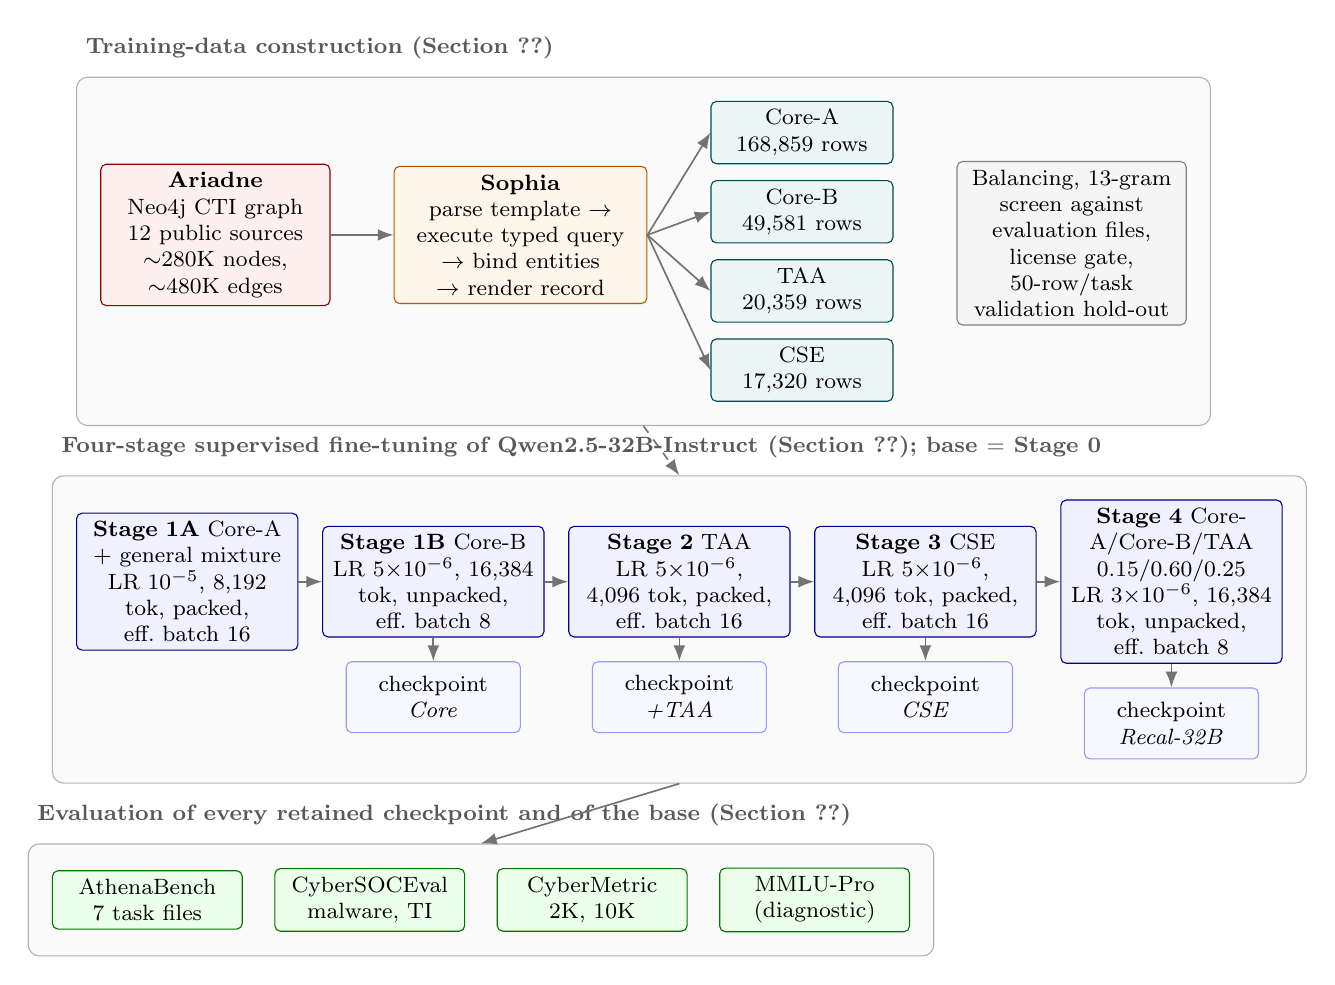
\begin{tikzpicture}[
  font=\footnotesize, >={Latex[length=2mm]}, node distance=3mm and 4mm,
  box/.style={draw, rounded corners=2pt, align=center, inner sep=3pt, minimum height=9mm},
  src/.style={box, fill=red!6, draw=red!55!black, text width=27mm},
  gen/.style={box, fill=orange!8, draw=orange!70!black, text width=30mm},
  shard/.style={box, fill=teal!8, draw=teal!60!black, text width=21mm, minimum height=7mm},
  stage/.style={box, fill=blue!6, draw=blue!55!black, text width=26mm},
  ev/.style={box, fill=green!8, draw=green!45!black, text width=22mm, minimum height=7mm},
  arr/.style={->, semithick, black!55}, grp/.style={draw=black!30, rounded corners=4pt, inner sep=3mm, fill=black!2},
  lbl/.style={font=\footnotesize\bfseries, text=black!65}]
\node[src] (ari) {\textbf{Ariadne}\\Neo4j CTI graph\\12 public sources\\$\sim$280K nodes, $\sim$480K edges};
\node[gen, right=8mm of ari] (sop) {\textbf{Sophia}\\parse template $\to$ execute typed query $\to$ bind entities $\to$ render record};
\node[shard, right=8mm of sop, yshift=13mm] (sa) {Core-A\\168,859 rows};
\node[shard, below=2mm of sa] (sb) {Core-B\\49,581 rows};
\node[shard, below=2mm of sb] (st) {TAA\\20,359 rows};
\node[shard, below=2mm of st] (sc) {CSE\\17,320 rows};
\node[box, fill=black!4, draw=black!50, text width=27mm, right=8mm of sb, yshift=-4mm] (scr) {Balancing, 13-gram screen against evaluation files, license gate, 50-row/task validation hold-out};
\draw[arr] (ari) -- (sop);
\foreach \s in {sa,sb,st,sc} \draw[arr] (sop.east) -- (\s.west);
\begin{scope}[on background layer]
 \node[grp, fit=(ari)(sop)(sa)(sc)(scr)] (g1) {};
\end{scope}
\node[lbl, above=1mm of g1.north west, anchor=south west] {Training-data construction (Section~\ref{sec:data})};
% stages
\node[stage, below=11mm of g1.south west, anchor=north west] (s1) {\textbf{Stage 1A} Core-A + general mixture\\LR $10^{-5}$, 8,192 tok, packed, eff.\ batch 16};
\node[stage, right=3mm of s1] (s1b) {\textbf{Stage 1B} Core-B\\LR $5{\times}10^{-6}$, 16,384 tok, unpacked, eff.\ batch 8};
\node[stage, right=3mm of s1b] (s2) {\textbf{Stage 2} TAA\\LR $5{\times}10^{-6}$, 4,096 tok, packed, eff.\ batch 16};
\node[stage, right=3mm of s2] (s3) {\textbf{Stage 3} CSE\\LR $5{\times}10^{-6}$, 4,096 tok, packed, eff.\ batch 16};
\node[stage, right=3mm of s3] (s4) {\textbf{Stage 4} Core-A/Core-B/TAA 0.15/0.60/0.25\\LR $3{\times}10^{-6}$, 16,384 tok, unpacked, eff.\ batch 8};
\draw[arr] (s1) -- (s1b); \draw[arr] (s1b) -- (s2); \draw[arr] (s2) -- (s3); \draw[arr] (s3) -- (s4);
\node[box, fill=blue!3, draw=blue!40, text width=20mm, below=3mm of s1b] (c1) {checkpoint\\\emph{Core}};
\node[box, fill=blue!3, draw=blue!40, text width=20mm, below=3mm of s2] (c2) {checkpoint\\\emph{+TAA}};
\node[box, fill=blue!3, draw=blue!40, text width=20mm, below=3mm of s3] (c3) {checkpoint\\\emph{CSE}};
\node[box, fill=blue!3, draw=blue!40, text width=20mm, below=3mm of s4] (c4) {checkpoint\\\emph{Recal-32B}};
\draw[arr] (s1b) -- (c1); \draw[arr] (s2) -- (c2); \draw[arr] (s3) -- (c3); \draw[arr] (s4) -- (c4);
\begin{scope}[on background layer]
 \node[grp, fit=(s1)(s4)(c1)(c4)] (g2) {};
\end{scope}
\node[lbl, above=1mm of g2.north west, anchor=south west] {Four-stage supervised fine-tuning of Qwen2.5-32B-Instruct (Section~\ref{sec:training}); base $=$ Stage 0};
% eval
\node[ev, below=11mm of g2.south west, anchor=north west] (e1) {AthenaBench\\7 task files};
\node[ev, right=4mm of e1] (e2) {CyberSOCEval\\malware, TI};
\node[ev, right=4mm of e2] (e3) {CyberMetric\\2K, 10K};
\node[ev, right=4mm of e3] (e4) {MMLU-Pro\\(diagnostic)};
\begin{scope}[on background layer]
 \node[grp, fit=(e1)(e4)] (g3) {};
\end{scope}
\node[lbl, above=1mm of g3.north west, anchor=south west] {Evaluation of every retained checkpoint and of the base (Section~\ref{sec:evaluation})};
\draw[arr] (g2.south) -- (g3.north);
\draw[arr, dashed] (g1.south) -- (g2.north);
\end{tikzpicture}}
\caption{Glaukopis pipeline as configured for the reported v21 release. Shard sizes are the realized post-screen training rows; stage settings are read from the release launchers. The general mixture in Stage 1A (T\"ulu-3 SFT and Alpaca) is not Sophia-generated and is not screened against the evaluation files.}\label{fig:pipeline}
\end{figure}

\begin{table}[!htbp]
\centering\footnotesize
\caption{Pipeline boundaries. Provenance is strongest for Sophia-materialized CTI targets; it should not be generalized to all auxiliary data or to unconstrained model completions.}\label{tab:boundaries}
\begin{tabularx}{\textwidth}{@{}p{2.4cm}XXX@{}}
\toprule Component & Input and transformation & Resulting artifact & Scope of assurance \\\midrule
Ariadne & Public CTI records normalized to typed entities and relations & Neo4j CTI snapshot & Source-linked facts; not proof of source completeness or correctness \\
Sophia & Expert-authored template, typed query, graph binding, rendering & Instruction, context, and target record with template identifier & Target traceable to the executed graph binding \\
Corpus preparation & Generation, balancing, $n$-gram screening, license gate, phase splitting & Core-A, Core-B, TAA, CSE, and validation shards & Dependent on covered files, fields, thresholds, and retained reports \\
Supervised training & Stage-specific shard mixture and optimizer configuration & Core, +TAA, CSE, Recal-32B checkpoints & Observable transitions; no isolated scheduling effect \\
Evaluation & Fixed task inputs, checkpoint, parser and scorer, serving settings & Predictions, per-item scores, run manifests & Reproducible only to the extent the run manifests and artifacts are retained \\\bottomrule
\end{tabularx}
\end{table}

\subsection{Typed-query materialization}
Sophia parses a declarative template, executes its typed graph query, binds the returned entities and relationships, and renders instruction records (Figure~\ref{fig:pipeline}). Templates support property access, relationship traversals, list expansion, hidden bindings, source disambiguation, and equality or inequality constraints. The following abbreviated pattern correlates a CVE with its weakness and attack pattern:
\begin{lstlisting}
Question: Correlate CVE, CWE, and CAPEC for a single vulnerability chain.
Answer: CVE {cve:CVE.id} impacts CAPEC {cap:cve.impacts>CAPEC.name}
and is categorized as weakness {cwe:cve.problemType>Weakness.name}.
CAPEC {cap.id} exploits weakness {cwe2:cap.exploits>Weakness.name}.
<*{force cwe.id=cwe2.id}*>
\end{lstlisting}
The hidden equality constraint requires the two traversals to resolve to the same weakness identifier. A reviewer can therefore inspect the binding rather than trust a separately synthesized answer. The example illustrates the materialization mechanism; it is not a new reasoning benchmark.

Negative constraints can generate examples that distinguish graph-supported from unsupported associations. However, absence of a relationship in an incomplete CTI graph is not necessarily evidence that the relationship is false in the world. Negative examples should be interpreted against the declared graph and schema, with a documented closed-world assumption where appropriate.

The generation workflow parses template manifests, materializes bindings, balances and deduplicates records, and serializes Alpaca-format JSON. Schema tests detect template references to absent graph labels, relationships, or properties. These tests can reveal incompatibilities but do not replace a semantic audit of source mappings. The combination provides content control and inspectability without establishing a measured reduction in all types of label error.

\subsection{Corpus scope and reproducibility}
The reported v21 release uses four production CTI shards (Core-A, Core-B, TAA, and CSE) and three validation shards holding out 50 rows per template family. The build reports record the realized sizes: the Core corpus contained 219,675 rows after balancing, of which 684 were removed by the $n$-gram screen (Section~\ref{sec:contamination}), 550 were held out for validation, and of the remaining 218,441 training rows 168,859 were assigned to Core-A and 49,581 to Core-B (the phase-split report accounts for all but one row); the TAA and CSE shards contained 20,359 and 17,320 training rows. Core-A is trained together with a general-purpose instruction mixture (T\"ulu-3 SFT and Alpaca-English; \citealp{lambert2024tulu3,taori2023alpaca}), which is neither Sophia-generated nor screened. Consequently, the statement ``every training example is graph-materialized'' applies to Sophia-generated CTI records only.

The architecture ports use the same serialized CTI release. Nevertheless, exact row-level regeneration was not fully seed-pinned in v21: graph-read order, sampling, and deduplication tie-breaks can vary, and the project's own replay experiments found that byte-identical templates did not reproduce per-task scores within the intended tolerance. Template identity alone therefore does not certify identical training rows. A reproducible release needs hashes of the serialized files, per-source graph snapshots, counts after each filter, and software versions, in addition to the templates.

\section{Multi-stage training configuration}\label{sec:training}
\subsection{Base model and the rationale for the stages}
The base is \code{Qwen/Qwen2.5-32B-Instruct} \citep{qwen2025qwen25}, chosen for three reasons: it is openly licensed for local deployment; at 32B parameters it serves in bfloat16 on two 80-GB GPUs, which is the hardware a mid-sized SOC can allocate; and its zero-shot scores on CyberMetric (90.2) and MMLU-Pro (69.0) are high enough that losses of general capability are measurable against a strong baseline rather than hidden by a weak one. Additional ports to Qwen2.5-14B-Instruct, Qwen3-30B-A3B-Thinking-2507 \citep{yang2025qwen3}, Meta-Llama-3.1-8B-Instruct \citep{grattafiori2024llama3}, and Foundation-Sec-8B-Instruct \citep{kassianik2025foundationsec} test whether the recipe transfers across architecture and size; the mixture-of-experts (MoE) port has 30.5B total and 3.3B active parameters per token.

The four-stage schedule in Table~\ref{tab:training} was not designed a priori. It is the configuration the project converged on over twenty earlier releases on smaller bases, in which single mixed passes repeatedly improved some AthenaBench tasks while leaving the multiple-choice and attribution tasks near their base values. The schedule separates concerns in the order of increasing narrowness. Stage 1A trains the broad CTI families (knowledge questions, multiple choice, SOC triage, compliance, and yes/no families) together with a general instruction mixture, so that the model first sees the domain vocabulary without losing instruction-following behavior. Stage 1B trains the four catalog-mapping schemas (mitigation sets, technique extraction, severity vectors, root cause) at a longer context length because their prompts embed full CVE and technique descriptions. Stage 2 drills threat-actor attribution, whose answer space (ATT\&CK groups and their aliases) is small and had resisted improvement inside the broad mixture. Stage 3 drills the SOC-style multiple-select format used by CyberSOCEval, whose answers are letter sets. Stage 4 revisits a mixture of the Stage-1 and Stage-2 shards at a low learning rate to recover capabilities displaced by the two narrow drills. Each stage therefore has a stated purpose, and Section~\ref{sec:results} tests whether that purpose was achieved; retaining the checkpoint after each stage is what makes the test possible.

Training uses LlamaFactory \citep{zheng2024llamafactory} with DeepSpeed ZeRO-3 and CPU offload \citep{rajbhandari2020zero}, an 8-bit AdamW optimizer, Liger kernels, gradient checkpointing, and bfloat16 precision on eight 80-GB H100 GPUs; these are the standard choices for full-parameter fine-tuning of a 32B model on one node and were not varied. Effective batch size is preserved by adjusting gradient accumulation to the GPU count. Each stage runs for one epoch over its shard, so the number of updates per stage is determined by the shard size and the effective batch.

\begin{table}[!htbp]
\centering\footnotesize
\caption{Canonical 32B training recipe read from the v21 launchers. Caps are the per-dataset \texttt{max\_samples} limits, not realized token counts. The general mixture is capped separately from Core-A because the limit applies per dataset. Wall-time budgets are the project's documented planning figures for eight H100 GPUs, not metered bills of the reported runs.}\label{tab:training}
\fitwidth{\begin{tabular}{@{}llrrrrll@{}}
\toprule Pass & Training input & Cap & Max.\ tokens & LR & Eff.\ batch & Packing & Budget (h) \\\midrule
1A & Core-A + T\"ulu-3 SFT + Alpaca & 240,000 & 8,192 & $1\times10^{-5}$ & 16 & on & \multirow{2}{*}{26--30} \\
1B & Core-B & 70,000 & 16,384 & $5\times10^{-6}$ & 8 & off & \\
2 & TAA & 33,000 & 4,096 & $5\times10^{-6}$ & 16 & on & 13--17 \\
3 & CSE & 33,000 & 4,096 & $5\times10^{-6}$ & 16 & on & 9--13 \\
4 & Core-A/Core-B/TAA at 0.15/0.60/0.25 & 3,600 per shard & 16,384 & $3\times10^{-6}$ & 8 & off & 3--4 \\\bottomrule
\end{tabular}}
\end{table}

Because the caps exceed the realized Core-B, TAA, and CSE shard sizes, those passes consume their shards in one epoch. In pass 1A the cap applies to the Sophia shard and to each auxiliary dataset separately, so the general mixture can contribute up to 240,000 rows alongside the 168,859 Core-A rows; the auxiliary share is therefore material to the forgetting discussion in Section~\ref{sec:results}. Stage 4 interleaves the three shards under the stated probabilities up to the per-shard cap, which yields about 6,000 interleaved examples. Neither repeated exposure nor actual token consumption can be inferred from the caps; sequence limits are maxima, not average lengths.

The alternative Stage-4 recipe developed for the 14B port uses learning rate $10^{-6}$, mixture probabilities 0.25/0.40/0.35, and a 2,400-example cap. Both Stage-4 variants were trained from the same CSE parent on the 32B base and both are evaluated below. Applying different Stage-4 mixtures and rates across architectures means that the complete training treatment is not byte-identical across every port.

\subsection{What changes between stages}
Table~\ref{tab:training} makes explicit that four quantities change together at a stage boundary: the training data, the maximum sequence length, whether short examples are packed into one sequence, and the learning rate. This co-variation is deliberate from an engineering standpoint (each shard has its own natural context length, and the narrow drills use a lower rate than the broad pass), but it means that a difference between two consecutive checkpoints is the effect of the whole configuration change, not of the data alone. We call the retained models \emph{cumulative checkpoints}: they reveal the effect of continuing training under each configured treatment, and they are not matched ablations. In particular, Core$\rightarrow$CSE without the attribution stage and a single-stage mixture with the same realized tokens and updates were not trained in this release. The necessity of Stage 2 and the superiority of four stages over one are therefore not established by the chain, and the article does not claim them. Section~\ref{sec:singlestage} reports the closest single-stage run in the project record.

\subsection{A single-stage reference run}\label{sec:singlestage}
Before the staged recipe, the project trained Qwen2.5-32B-Instruct in a single stage on an earlier Sophia corpus (release v7, 26 April 2026): 180,533 CTI rows covering the broad knowledge, multiple-choice, attribution, and catalog-mapping families together with a small general instruction set, for three epochs at learning rate $10^{-5}$, sequence length 4,096 with packing, and effective batch 16. Its update budget (three passes over 180,533 rows) is comparable to the staged chain's (one pass over each of 168,859, 49,581, 20,359, and 17,320 Sophia rows plus the general mixture and the $\approx$6,000-row Stage 4). Both runs were evaluated with the same harness and task files, on different dates; the single-stage run predates the Canonical attribution task and MMLU-Pro, so Table~\ref{tab:singlestage} compares the two on the measures both share, using a Classic-only attribution convention for both rows. The single-stage run is not a matched control: its corpus lacks the CSE letter-set family and the glossary-sourced multiple-choice family that were added later, and its templates differ in detail from the release templates. It is, however, the most informative comparison the record contains, and it is reported here so that the reader can judge the schedule's contribution rather than infer it.

\begin{table}[!htbp]
\centering\footnotesize
\caption{Single-stage reference run (Qwen2.5-32B-Instruct, release v7 corpus, one pass) against the base model and the staged chain's final checkpoint, on the measures all three share. $A_{\mathrm{Cl}}$ is the AthenaBench mean with Classic attribution only; $B_{\mathrm{Cl}}$ is the three-benchmark mean built on it. Canonical attribution and MMLU-Pro were not evaluated for the v7 run. Single evaluations; from the project's results workbook.}\label{tab:singlestage}
\fitwidth{\begin{tabular}{@{}lrrrrrrrrrr@{}}
\toprule Model & CKT & ATE & RCM & RMS & VSP & TAA Cl. & $A_{\mathrm{Cl}}$ & $C$ & $Y$ & $B_{\mathrm{Cl}}$ \\\midrule
Base & 52.9 & 18.2 & 59.5 & 7.6 & 78.8 & 48.0 & 44.2 & 42.6 & 90.2 & 59.0 \\
Single-stage (v7 corpus, 3 epochs) & 71.0 & 57.4 & 62.1 & 68.5 & 83.4 & 52.5 & 65.8 & 39.6 & 88.6 & 64.7 \\
Staged chain, Recal-32B (v21) & 75.5 & 65.8 & 67.1 & 62.5 & 77.8 & 50.5 & 66.5 & 42.6 & 89.8 & 66.3 \\\bottomrule
\end{tabular}}
\end{table}

The two fine-tuned runs are close on the aligned benchmark (65.8 against 66.5 on $A_{\mathrm{Cl}}$) and differ by task: the staged chain is ahead on CKT ($+4.5$), ATE ($+8.4$), and RCM ($+5.0$), the single-stage run is ahead on RMS ($+6.0$), VSP ($+5.6$), and Classic attribution ($+2.0$), and on the two benchmarks built by other groups the staged chain holds the base model's level where the single-stage run loses three points on CyberSOCEval. Because the corpora differ, none of these differences can be attributed to the schedule. What the comparison does show is that most of the gain over the base model (from 44.2 to the mid-60s on $A_{\mathrm{Cl}}$) is obtained by a single pass over Sophia-generated data, and that the staged recipe's distinctive effects are the ones examined in Section~\ref{sec:results}: it reaches the aligned tasks the single pass did not (CKT, ATE) and it introduces regressions the single pass did not have (VSP). A matched control, defined as one pass over the union of the v21 shards with the same realized tokens and updates as the chain, remains the experiment that would settle the scheduling question; its cost is bounded by the chain's own budget in Table~\ref{tab:training}.

\section{Evaluation protocol}\label{sec:evaluation}
\subsection{Task portfolio, scorers, and run records}
AthenaBench evaluates CTI knowledge (CKT), attack-technique extraction (ATE), root-cause mapping (RCM), risk-mitigation strategy (RMS), vulnerability-severity prediction (VSP), and threat-actor attribution (TAA) in Classic and Canonical forms \citep{alam2025athenabench}. CyberSOCEval supplies malware-analysis and threat-intelligence-reasoning tasks \citep{deason2025cybersoceval}; CyberMetric supplies cybersecurity multiple-choice evaluation at the 2K and 10K tiers \citep{tihanyi2024cybermetric}; MMLU-Pro is a general-task diagnostic \citep{wang2024mmlupro}. Table~\ref{tab:portfolio} lists the item counts and the scorer that the harness applies to each task, read from the evaluation code. The scorers differ in kind, so task scores should not all be called accuracy or treated as calibrated probabilities of operational success.

\begin{table}[!htbp]
\centering\footnotesize
\caption{Evaluation portfolio as executed for the 32B chain. Item counts are from the run manifests; scorer definitions are from the evaluation code. TAA and RMS ``combined'' scores award full credit for a strict match and half credit for a plausible match (an alias or related group for TAA; a mitigation from the technique's neighbourhood for RMS).}\label{tab:portfolio}
\begin{tabularx}{\textwidth}{@{}lrX@{}}
\toprule Task & Items & Per-item score used in the aggregates \\\midrule
CKT (multiple choice) & 3,000 & 1 if the option letter matches \\
RCM & 2,000 & 1 if the CWE identifier matches exactly \\
VSP & 2,000 & $1-|s_{\text{pred}}-s_{\text{gold}}|/7.7$, with $s$ the CVSS v3.1 base score of the parsed vector \citep{first2019cvss}; unparseable vectors are excluded (two of 2,000 for the final checkpoint) \\
ATE & 500 & 1 if the technique matches at the parent-technique level (sub-technique suffix ignored) \\
RMS & 500 & Set F1 over predicted mitigation identifiers; combined variant credits neighbourhood mitigations at half weight \\
TAA Classic & 100 & 1 alias-connected, 0.5 related group, 0 otherwise \\
TAA Canonical & 133 & 1 if the canonical group name or G-code appears, 0.5 if another alias of the group appears, 0 otherwise \\
CyberSOCEval malware / TI & 609 / 588 & Jaccard similarity between predicted and gold option-letter sets; strict accuracy is Jaccard $=1$; unparseable responses are excluded from both denominators \\
CyberMetric 2K / 10K & 2,000 / 10,180 & 1 if the option letter matches \\
MMLU-Pro & 12,032 & 1 if the extracted option letter matches (zero-shot chain-of-thought prompt) \\\bottomrule
\end{tabularx}
\end{table}

Local checkpoints were served with vLLM \citep{kwon2023vllm} on two H100 GPUs at batch size 32 (64 for MMLU-Pro), and hosted references used the same harness through provider APIs \citep{glaukopis2026software}. The run manifests date the CTI evaluations of the five 32B checkpoints to 20--21 May 2026 and the MMLU-Pro evaluations to 23--26 May 2026. Each score is a single evaluation of a single training run. Item-level prediction and score files were retained for the five fine-tuned checkpoints and are the basis of the bootstrap and error analyses below; the corresponding files for the base model and the hosted references were not retained, so paired statistics involving them are not reported.

\subsection{Baselines and reference models}\label{sec:baselines}
Five kinds of comparison are reported, each controlling something different.
\begin{enumerate}
\item \emph{The base model}, Qwen2.5-32B-Instruct, evaluated zero-shot with the same prompts. Every fine-tuned score is read against it; this is the only comparison in which the architecture, parameter count, and serving configuration are held fixed.
\item \emph{A security-specialized open model}, Foundation-Sec-8B-Instruct \citep{kassianik2025foundationsec}, an 8B Llama-3.1 derivative continued-pretrained on cybersecurity text and instruction-tuned by its authors. It represents the alternative of adopting an existing domain model rather than specializing one, and it is also used as a base for one of the ports (Table~\ref{tab:ports}).
\item \emph{Six hosted frontier models}: GPT-5.5 and GPT-5.2 \citep{openai2026gpt55,openai2025gpt52}, DeepSeek-V4-Pro and DeepSeek-V3.2-Exp \citep{deepseek2026v4,deepseek2025v32exp}, and Gemini-3-Flash-Preview and Gemini-2.5-Flash \citep{google2025gemini3flash,comanici2025gemini25}, evaluated through provider APIs with the same harness and prompts (Table~\ref{tab:frontier}). They bound what is achievable without local deployment and without specialization.
\item \emph{A single-stage fine-tuning run} on the same base from the project record (Section~\ref{sec:singlestage}), which bounds how much of the gain requires the stage schedule.
\item \emph{Four architecture ports} of the same recipe (Table~\ref{tab:ports}), which test transfer across model families and sizes.
\end{enumerate}
No comparison with other published CTI fine-tuning systems is made at the level of scores: CyberPal.AI and SecKnowledge \citep{levi2025cyberpal} and the systems in Table~\ref{tab:positioning} do not release weights evaluated on this suite, so a score comparison would require retraining them under our protocol, which was outside the project's budget. Their comparison in Table~\ref{tab:positioning} is therefore architectural, and we say so.

\subsection{Evaluation independence}\label{sec:independence}
The three CTI benchmarks differ in their independence from the training data. AthenaBench is aligned by design: Core-B trains the schemas assessed by its mapping and mitigation tasks, Stage 2 targets its attribution task, and Core-A includes multiple-choice families of the kind its knowledge task uses. It was also built by a team that includes two of the present authors. CyberSOCEval was built by Meta and CrowdStrike and CyberMetric by an unrelated academic group; neither was consulted when the templates were written, although Stage 3 does target CyberSOCEval's multiple-select answer format. MMLU-Pro is unrelated to the domain. The results are therefore reported in three tiers: AthenaBench measures whether the model learned the schemas it was trained on; CyberSOCEval and CyberMetric measure whether that learning transfers to CTI questions written by others; and MMLU-Pro measures what the specialization cost. Section~\ref{sec:overlap} quantifies, for AthenaBench, how often a test item's entities and gold answer occur in a training row, and reports scores on the items where they do not. Sharing public catalogs is appropriate for measuring public-catalog competence, but it does not establish generalization to unseen facts, new incidents, or private SOC telemetry, and an entity-disjoint or temporally held-out incident set remains the test that would.

\subsection{Contamination screening: what was run and what it covered}\label{sec:contamination}
Before training, each shard was scanned for verbatim overlap with the evaluation files. The filter lowercases alphanumeric word tokens and indexes distinct 13-word sequences; a single shared sequence flags a row for audit, and at least 50 shared sequences with one indexed evaluation record trigger removal. Table~\ref{tab:ngram} reports the retained build reports. The Core corpus had 34,897 flagged rows (15.9\%), almost all against the AthenaBench RCM, ATE, RMS, and VSP files, and 684 rows (0.3\%) were removed, chiefly VSP and RCM template rows that reproduced CVE descriptions at length. The TAA shard had no flagged row; the CSE shard had 41 flagged rows and none removed. Flagged-but-retained rows share between one and 49 thirteen-grams with an evaluation record; for a record of $L$ tokens the number of distinct 13-grams is at most $L-12$, so a complete duplicate of an evaluation record shorter than 62 tokens can never reach the removal threshold. The retained-overlap band is therefore a documented property of the method, not evidence that a particular test item was memorized.

\begin{table}[!htbp]
\centering\footnotesize
\caption{Verbatim 13-gram screen as executed in the v21 build (build reports, May 2026). ``Flagged'' rows share at least one 13-gram with an indexed evaluation record and are shown by their maximum number of shared 13-grams with a single record; rows at 50 or more were removed. The index held 808,440 distinct 13-grams from 18 files.}\label{tab:ngram}
\fitwidth{\begin{tabular}{@{}lrrrrrrrrr@{}}
\toprule & & \multicolumn{6}{c}{Flagged rows by maximum shared 13-grams} & & \\\cmidrule(lr){3-8}
Shard & Scanned & 1 & 2--4 & 5--12 & 13--24 & 25--49 & $\ge$50 (removed) & Flagged total & Retained \\\midrule
Core & 219,675 & 6,641 & 10,952 & 6,656 & 3,165 & 6,799 & 684 & 34,897 (15.9\%) & 218,991 \\
TAA & 20,509 & 0 & 0 & 0 & 0 & 0 & 0 & 0 & 20,509 \\
CSE & 17,670 & 24 & 17 & 0 & 0 & 0 & 0 & 41 (0.2\%) & 17,670 \\\bottomrule
\end{tabular}}
\end{table}

Coverage is narrower than the project documentation implies. The 18 indexed files were the AthenaBench task files, the CyberMetric files, and two operational CVE and URL feeds. The CyberSOCEval question files are fetched into the evaluation directory at run time and were not present when the shards were built, so the CSE shard was screened only against AthenaBench and CyberMetric; the CTIBench tab-separated files were also outside the JSON glob. The auxiliary T\"ulu-3 and Alpaca mixtures were not screened at all, and base-model pretraining contamination is outside scope. Index keys use the file basename and row index, and only selected text fields are extracted. Hash-based exact deduplication, full-path identifiers, and a CyberSOCEval scan should be added before ``decontaminated'' is used without qualification.

\subsection{Entity and gold-fact overlap}\label{sec:overlap}
Verbatim screening cannot detect the case that matters most for a graph-generated corpus: a training row that states the evaluated fact in different words. We therefore measured, for each AthenaBench task, whether the evaluation item's entities and its gold answer co-occur in a single training row (Table~\ref{tab:overlap}). Technique identifiers are a bounded catalog and every ATE and RMS target appears in training, as expected for catalog competence. Of the 2,000 RCM items, 660 CVE identifiers appear somewhere in the Core shard and 137 items (6.9\%) have their exact CVE-to-CWE gold pair stated in one row. For VSP, 446 CVE identifiers appear but only seven items have their exact CVSS vector co-located with the identifier. For RMS, 273 of 500 items (54.6\%) have the technique's full gold mitigation set listed in one row, because catalog-listing templates enumerate a technique's mitigations. For Canonical TAA, 38 of 133 alias-to-group pairs are stated in a Core row.

\begin{table}[!htbp]
\centering\footnotesize
\caption{Overlap between the v21 training shards and AthenaBench items, and the final checkpoint's mean item score on overlapping versus non-overlapping items. ``Gold fact in one row'' means that the item's identifying entity and its complete gold answer co-occur in a single training row of the Core shard (Core, TAA, and CSE shards for Canonical TAA). Scores are the per-item metrics of Table~\ref{tab:portfolio}.}\label{tab:overlap}
\fitwidth{\begin{tabular}{@{}lrrrrr@{}}
\toprule Task & Items & Entity in training & Gold fact in one row & Recal-32B: fact in training & Recal-32B: fact absent \\\midrule
RCM & 2,000 & 660 (33.0\%) & 137 (6.9\%) & 66.4 ($n{=}137$) & 64.3 ($n{=}1{,}340$)$^{a}$ \\
VSP & 2,000 & 446 (22.3\%) & 7 (0.4\%) & 77.4 ($n{=}445$)$^{b}$ & 77.9 ($n{=}1{,}553$) \\
ATE & 500 & 500 (100\%) & n/a & 70.5 (top tertile)$^{c}$ & 62.3 (bottom tertile) \\
RMS & 500 & 500 (100\%) & 273 (54.6\%) & 53.8 ($n{=}273$) & 73.1 ($n{=}227$) \\
TAA Canonical & 133 & 40 aliases (30.1\%) & 38 (28.6\%) & 7.9 ($n{=}38$) & 1.6 ($n{=}93$) \\\bottomrule
\end{tabular}}\par\smallskip
{\scriptsize $^{a}$Items whose CVE appears without the gold pair score 74.2 ($n{=}523$). $^{b}$CVE present in training (any row) versus absent. $^{c}$Items grouped by how often the gold technique occurs in training rows (tertile cuts at 156 and 298 rows; middle tertile 64.7).\par}
\end{table}

The subset scores do not show the pattern expected from memorization of leaked facts. RCM items whose gold pair appears in training score within about two points of items whose CVE never appears; RMS items whose full mitigation set appears in training score lower, because those are the techniques with large mitigation sets on which set-F1 is hardest; VSP is unchanged. Two tasks do track exposure: ATE accuracy rises with the training frequency of the gold technique, and at the +TAA checkpoint Canonical-TAA items whose alias-to-group mapping appears in training score 52.6 against 30.6 for the remainder. These are the expected signatures of catalog competence rather than of test-item leakage, and they identify attribution as the task most dependent on explicit fact exposure. Semantic paraphrases of evaluation narratives, reused public facts, and benchmark-guided recipe selection remain uncontrolled; an entity-disjoint or temporally held-out incident set is still required for an out-of-sample claim.

\subsection{Explicit aggregation and the corrected attribution convention}\label{sec:aggregation}
To avoid hiding the Canonical-TAA regression, we define a balanced attribution score, an AthenaBench macro-score, and a three-benchmark mean:
\begin{align}
 \Tbal &= \tfrac12\,(T_{\mathrm{Classic}}+T_{\mathrm{Canonical}}),\\
 \Abal &= \tfrac16\,(K+E+R+M+V+\Tbal),\\
 \Bbal &= \tfrac13\,(\Abal+C+Y).
\end{align}
Here $K,E,R,M,V$ denote CKT, ATE, RCM, combined RMS, and VSP; $Y$ is the mean of the two CyberMetric tiers; and $C$ is the CyberSOCEval composite used throughout the project's results workbook for every row, including the hosted references, namely the mean of malware strict accuracy, malware Jaccard score, and threat-intelligence strict accuracy. That composite omits the threat-intelligence Jaccard score; a symmetric four-metric mean would change $\Bbal$ by at most 2.7 points for the rows reported here and would not change the base-to-final gain by more than 0.2 points. We retain the project convention so that every row is computed identically and state it explicitly.

Two further aggregates appear in the tables. The \emph{ten-test mean} averages CKT, ATE, RCM, strict RMS F1, VSP, $\Tbal$, the two strict CyberSOCEval accuracies, and the two CyberMetric tiers with equal weight; it is the project's long-standing leaderboard number and is reported for continuity. MMLU-Pro is never averaged into a CTI score, because a general-task diagnostic and a domain score measure different things. Readers comparing these values with the project's earlier conference draft should note that the draft's AthenaBench composite for the fine-tuned checkpoints used Classic attribution alone (66.3 for the final checkpoint, 59.0 for the base); under the uniform $\Tbal$ convention those values are 65.0 and 57.7, and the gain is unchanged at 7.3 points. Every number in this article was recomputed from the per-item artifacts and run manifests under the conventions stated here.

\subsection{Uncertainty}\label{sec:uncertainty}
For the five fine-tuned checkpoints we computed 95\% percentile bootstrap intervals by resampling evaluation items with replacement (2,000 replicates), independently within each task and jointly for the aggregates \citep{efron1993bootstrap}. Differences between checkpoints use the same resampled items for both members of a pair, so they are paired estimates. These intervals quantify item-sampling uncertainty for a fixed trained model only. They say nothing about the variance of training itself, which would require independently seeded runs of the same recipe, and clustered items (for example, several CyberSOCEval questions drawn from one report) are treated as independent, which makes the intervals slightly optimistic for that benchmark.

\section{Results: adaptation, interference, and transfer}\label{sec:results}
\subsection{The canonical 32B chain}
Table~\ref{tab:stage} reports the task scores of the base model and the five retained checkpoints together with the aggregates of Section~\ref{sec:aggregation}; the ten-test means of the chain are 61.6, 61.7, 62.4, 62.4, and 62.9 against 49.6 for the base. Relative to the base, the final checkpoint improves ATE by 47.6 points, RMS by 54.9, CKT by 22.6, and RCM by 7.6; VSP decreases by 1.0 point, and MMLU-Pro by 11.6. The balanced AthenaBench score rises from 40.3 to 62.6 and the three-benchmark mean from 57.7 to 65.0. The item-bootstrap interval for the final checkpoint's $\Bbal$ is 64.1--66.0 and for $\Abal$ is 61.5--63.7; no paired interval with the base is available, but an unpaired normal approximation from the base's reported accuracies and item counts gives half-widths below 2.5 points for every accuracy task except ATE (3.4), so the base-to-final gain is far outside item-sampling noise.

\begin{table}[!htbp]
\centering\scriptsize
\setlength{\tabcolsep}{3.3pt}
\caption{Task scores and aggregates for the canonical Qwen2.5-32B chain (single evaluation per checkpoint; 0--100 scale). $\Abal$ and $\Bbal$ follow Section~\ref{sec:aggregation} and are computed from the displayed rounded task scores; recomputing them from unrounded item scores changes them by at most 0.1. Recal-14B is the alternative Stage-4 recipe trained from the same CSE parent. The last row gives the half-width (larger side) of the final checkpoint's 95\% item-bootstrap interval.}\label{tab:stage}
\setlength{\tabcolsep}{2.8pt}
\fitwidth{\begin{tabular}{@{}lrrrrrrrrrrrr@{}}
\toprule Checkpoint & CKT & ATE & RCM & RMS & VSP & TAA Cl. & TAA Can. & $C$ & $Y$ & MMLU-Pro & $\Abal$ & $\Bbal$ \\\midrule
Base & 52.9 & 18.2 & 59.5 & 7.6 & 78.8 & 48.0 & 2.0 & 42.6 & 90.2 & 69.0 & 40.3 & 57.7 \\
Core & 72.9 & 67.2 & 69.8 & 63.8 & 83.1 & 46.5 & 18.4 & 31.1 & 89.6 & 59.2 & 64.9 & 61.9 \\
+TAA & 75.4 & 63.4 & 69.0 & 62.9 & 83.5 & 47.0 & 36.8 & 29.8 & 89.4 & 58.2 & 66.0 & 61.7 \\
CSE & 72.5 & 63.4 & 67.7 & 63.7 & 78.9 & 53.5 & 3.4 & 42.0 & 88.8 & 54.2 & 62.4 & 64.4 \\
Recal-14B & 76.0 & 61.6 & 68.3 & 63.6 & 75.7 & 50.5 & 5.6 & 42.4 & 89.2 & 54.6 & 62.2 & 64.6 \\
Recal-32B & 75.5 & 65.8 & 67.1 & 62.5 & 77.8 & 50.5 & 3.4 & 42.6 & 89.8 & 57.4 & 62.6 & 65.0 \\
\multicolumn{1}{@{}r}{\scriptsize 95\% half-width} & $\pm$1.6 & $\pm$4.4 & $\pm$2.0 & $\pm$3.4 & $\pm$1.1 & $\pm$5.5 & $\pm$3.0 & $\pm$2.5 & $\pm$0.7 & $\pm$1.0 & $\pm$1.1 & $\pm$1.0 \\
\bottomrule
\end{tabular}}
\end{table}

The cross-benchmark gain is not spread across the three benchmark families. The AthenaBench term contributes $+7.4$ to the 7.3-point change in $\Bbal$, the CyberSOCEval term contributes zero (42.6 to 42.6), and the CyberMetric term contributes $-0.1$. The entire positive contribution therefore comes from the benchmark that the training shards target most directly. This is useful evidence of schema adaptation, not evidence of uniform gains across independently targeted CTI workloads.

Why the two external benchmarks do not move is explained by what they measure. CyberMetric is a knowledge test on which the base model already scores 90.2; the training data adds catalog facts the base largely knows, and the fine-tuned checkpoints neither gain nor lose more than a point, which is the expected result of specialization that does not damage general security knowledge. CyberSOCEval's composite is flat for a different reason: its two components move in opposite directions across the chain (Figure~\ref{fig:trajectories}). Malware-analysis accuracy falls from 24.1 to 7.8 after Stage 1, when the model has learned to answer with a single technique or identifier and no longer produces the multi-select letter set the task requires, and recovers to 26.4 only after Stage 3 teaches that format; threat-intelligence accuracy follows the same path (49.9 to 41.1 to 48.9) without quite regaining the base. The final composite therefore reflects a format recovered rather than reasoning gained, and the benchmark should not be read as showing transfer of CTI knowledge from the training data. The improvement on AthenaBench is itself concentrated in the tasks whose answer is a catalog identifier chosen from a bounded space (RMS, ATE, CKT), which is where a model that has been shown the catalog in the right format gains most and where a benchmark-aligned corpus is most likely to help; RCM, whose answer requires judging a free-text description, improves by 7.6 points, and VSP, which requires judging eight metrics, does not improve at all.

\subsection{What each transition reveals}
Figure~\ref{fig:trajectories} and Table~\ref{tab:paired} show the transitions with their paired intervals. The attribution stage raises Canonical TAA from 18.4 to 36.8 ($+18.4$, interval $+12.4$ to $+24.4$) and CKT by 2.6 points, with no reliable change elsewhere; under the balanced aggregation, AthenaBench peaks at this checkpoint (66.0), not at the released one.

\begin{figure}[!htbp]
\centering
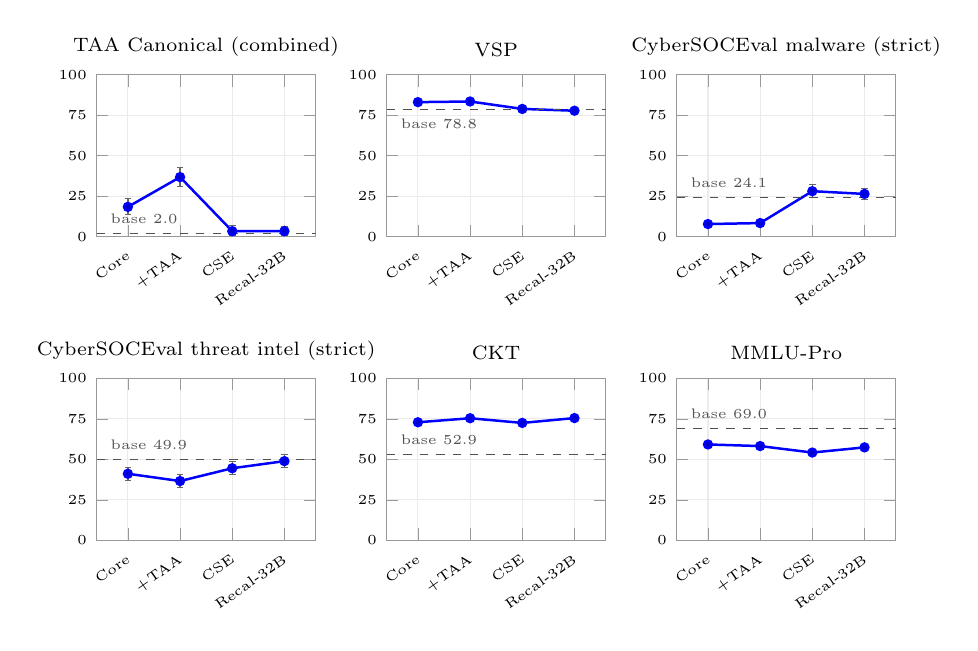
\begin{tikzpicture}
\begin{groupplot}[
  %% vertical sep must clear the rotated x tick labels of the upper row; at 13mm
  %% the lower row's titles printed on top of them.
  group style={group size=3 by 2, horizontal sep=9mm, vertical sep=18mm},
  width=0.36\textwidth, height=0.3\textwidth,
  ymin=0, ymax=100, ytick={0,25,50,75,100},
  xmin=-0.6, xmax=3.6, xtick={0,1,2,3}, xticklabels={Core,+TAA,CSE,Recal-32B}, x tick label style={font=\tiny, rotate=35, anchor=north east},
  y tick label style={font=\tiny}, title style={font=\scriptsize, yshift=-1mm},
  axis line style={black!40}, tick style={black!40}, grid=major, grid style={black!8},
  every axis plot/.append style={seriesblue, mark=*, mark size=1.4pt, line width=0.9pt, error bars/y dir=both, error bars/y explicit, error bars/error bar style={black!60, line width=0.5pt}, error bars/error mark options={black!60, rotate=90, mark size=1.2pt}}]
\nextgroupplot[title={TAA Canonical (combined)}]
\addplot coordinates {(0,18.4)+=(0,5.3)-=(0,4.9) (1,36.8)+=(0,5.7)-=(0,5.6) (2,3.4)+=(0,3.4)-=(0,2.6) (3,3.4)+=(0,3.0)-=(0,2.6)};
\draw[refgray, dashed] (axis cs:-0.6,2.0) -- (axis cs:3.6,2.0) node[pos=0.02, above right, font=\tiny, text=refgray] {base 2.0};
\nextgroupplot[title={VSP}]
\addplot coordinates {(0,83.1)+=(0,0.7)-=(0,0.7) (1,83.5)+=(0,0.6)-=(0,0.7) (2,78.9)+=(0,1.0)-=(0,1.0) (3,77.8)+=(0,1.1)-=(0,1.1)};
\draw[refgray, dashed] (axis cs:-0.6,78.8) -- (axis cs:3.6,78.8) node[pos=0.02, below right, font=\tiny, text=refgray] {base 78.8};
\nextgroupplot[title={CyberSOCEval malware (strict)}]
\addplot coordinates {(0,7.8)+=(0,2.3)-=(0,2.2) (1,8.4)+=(0,2.4)-=(0,2.2) (2,28.1)+=(0,4.1)-=(0,4.0) (3,26.4)+=(0,3.6)-=(0,3.5)};
\draw[refgray, dashed] (axis cs:-0.6,24.1) -- (axis cs:3.6,24.1) node[pos=0.02, above right, font=\tiny, text=refgray] {base 24.1};
\nextgroupplot[title={CyberSOCEval threat intel (strict)}]
\addplot coordinates {(0,41.1)+=(0,3.9)-=(0,4.0) (1,36.6)+=(0,3.8)-=(0,3.9) (2,44.5)+=(0,4.2)-=(0,4.1) (3,48.9)+=(0,4.1)-=(0,4.2)};
\draw[refgray, dashed] (axis cs:-0.6,49.9) -- (axis cs:3.6,49.9) node[pos=0.02, above right, font=\tiny, text=refgray] {base 49.9};
\nextgroupplot[title={CKT}]
\addplot coordinates {(0,72.9)+=(0,1.5)-=(0,1.6) (1,75.4)+=(0,1.6)-=(0,1.6) (2,72.5)+=(0,1.6)-=(0,1.6) (3,75.5)+=(0,1.6)-=(0,1.5)};
\draw[refgray, dashed] (axis cs:-0.6,52.9) -- (axis cs:3.6,52.9) node[pos=0.02, above right, font=\tiny, text=refgray] {base 52.9};
\nextgroupplot[title={MMLU-Pro}]
\addplot coordinates {(0,59.2)+=(0,0.9)-=(0,0.8) (1,58.2)+=(0,0.9)-=(0,0.9) (2,54.2)+=(0,0.9)-=(0,0.9) (3,57.4)+=(0,1.0)-=(0,0.9)};
\draw[refgray, dashed] (axis cs:-0.6,69.0) -- (axis cs:3.6,69.0) node[pos=0.02, above right, font=\tiny, text=refgray] {base 69.0};
\end{groupplot}
\end{tikzpicture}
\caption{Six task scores across the retained checkpoints of the canonical chain (points) with 95\% item-bootstrap intervals (bars) and the base model's score as a dashed reference. Intervals for the base are not available. The panels share one 0--100 axis; Stage 3 (CSE) raises the SOC-style tasks and collapses canonical attribution and part of VSP, and Stage 4 recovers CKT and MMLU-Pro but neither attribution nor VSP.}\label{fig:trajectories}
\end{figure}

\begin{table}[!htbp]
\centering\scriptsize
\setlength{\tabcolsep}{3.5pt}
\caption{Paired differences between checkpoints (later minus earlier) with 95\% paired item-bootstrap intervals; intervals that exclude zero are marked with an asterisk. These quantify item-sampling uncertainty for the specific trained models, not training-seed variance.}\label{tab:paired}
\fitwidth{\begin{tabular}{@{}lrrrr@{}}
\toprule Metric & +TAA $-$ Core & CSE $-$ +TAA & Recal-32B $-$ CSE & Recal-32B $-$ Core \\\midrule
CKT & $+2.6$ \ci{+1.0}{+4.2}* & $-3.0$ \ci{-4.5}{-1.4}* & $+3.1$ \ci{+1.5}{+4.6}* & $+2.7$ \ci{+1.1}{+4.2}* \\
ATE & $-3.8$ \ci{-7.6}{+0.2} & $0.0$ \ci{-4.8}{+4.6} & $+2.4$ \ci{-2.4}{+7.2} & $-1.4$ \ci{-5.2}{+2.8} \\
RCM & $-0.8$ \ci{-1.3}{-0.2}* & $-1.3$ \ci{-2.2}{-0.4}* & $-0.6$ \ci{-1.9}{+0.8} & $-2.7$ \ci{-3.9}{-1.5}* \\
RMS & $-1.0$ \ci{-3.3}{+1.6} & $+0.9$ \ci{-1.5}{+3.3} & $-1.2$ \ci{-3.9}{+1.5} & $-1.3$ \ci{-4.0}{+1.4} \\
VSP & $+0.3$ \ci{-0.1}{+0.7} & $-4.5$ \ci{-5.5}{-3.5}* & $-1.1$ \ci{-2.3}{0.0} & $-5.3$ \ci{-6.4}{-4.2}* \\
TAA Classic & $+0.5$ \ci{-5.0}{+6.0} & $+6.5$ \ci{+1.0}{+12.5}* & $-3.0$ \ci{-8.5}{+2.5} & $+4.0$ \ci{-1.5}{+9.5} \\
TAA Canonical & $+18.4$ \ci{+12.4}{+24.4}* & $-33.5$ \ci{-39.8}{-27.1}* & $0.0$ \ci{-3.0}{+2.6} & $-15.0$ \ci{-20.7}{-9.4}* \\
CSE malware (strict) & $+0.6$ \ci{-0.4}{+1.6} & $+19.7$ \ci{+15.3}{+24.2}* & $-1.8$ \ci{-4.5}{+1.0} & $+18.6$ \ci{+14.9}{+22.5}* \\
CSE threat intel (strict) & $-4.5$ \ci{-6.7}{-2.3}* & $+7.9$ \ci{+3.3}{+12.4}* & $+4.4$ \ci{+1.8}{+7.2}* & $+7.9$ \ci{+3.6}{+12.0}* \\
CyberMetric 10K & $-0.3$ \ci{-0.6}{0.0} & $-0.3$ \ci{-0.7}{+0.1} & $+0.8$ \ci{+0.5}{+1.2}* & $+0.2$ \ci{-0.2}{+0.6} \\
MMLU-Pro & $-1.0$ \ci{-1.7}{-0.4}* & $-4.0$ \ci{-4.8}{-3.2}* & $+3.2$ \ci{+2.5}{+3.9}* & $-1.8$ \ci{-2.6}{-1.1}* \\
$\Abal$ & $+1.1$ \ci{+0.1}{+2.2}* & $-3.6$ \ci{-4.8}{-2.3}* & $+0.2$ \ci{-0.9}{+1.3} & $-2.3$ \ci{-3.4}{-1.1}* \\
$\Bbal$ & $-0.1$ \ci{-0.6}{+0.4} & $+2.7$ \ci{+1.7}{+3.8}* & $+0.6$ \ci{-0.2}{+1.4} & $+3.2$ \ci{+2.2}{+4.2}* \\
\bottomrule
\end{tabular}}
\end{table}

The Core transition produces the largest changes in the chain because it is the only stage that teaches the four mapping schemas: RMS rises from 7.6 to 63.8 and ATE from 18.2 to 67.2 chiefly because the base model, asked for mitigation identifiers or a technique code, produces prose or the wrong identifier family, whereas after Core-B it produces the requested identifiers in the requested final-line format. The gain is therefore partly format compliance and partly catalog recall, and the record does not separate the two. The attribution stage behaves as intended: it is the only transition that moves Canonical TAA upward, and Table~\ref{tab:taataxonomy} shows how, by converting ``wrong but known group'' answers (78 to 32) into correct-group answers under an alias (31 to 64) and exact answers (9 to 17). The model learns which group the tradecraft belongs to before it learns the group's canonical name.

Stage 3 raises CyberSOCEval malware strict accuracy by 19.7 points and threat-intelligence accuracy by 7.9 relative to +TAA, but Canonical TAA falls by 33.5 points (interval $-39.8$ to $-27.1$), VSP by 4.5, CKT by 3.0, and MMLU-Pro by 4.0, all outside their intervals. Classic TAA rises by 6.5. Stage 3 also introduces parsing failures: 17.1\% of malware responses could not be parsed at the CSE checkpoint against 0.7\% at Core, and because the scorer excludes unparseable responses, the malware accuracy with failures counted as wrong is 23.3 rather than 28.1. Section~\ref{sec:cseshard} shows that these effects follow from the content of the CSE shard. The recovery stage does not meet its objective of restoring VSP: 77.8 is below both its CSE parent (78.9) and the base (78.8), and Canonical TAA stays at 3.4. It does recover CKT ($+3.1$), MMLU-Pro ($+3.2$), threat-intelligence accuracy ($+4.4$), and both CyberMetric tiers, and it lowers the malware parsing-failure rate to 5.9\%. The resulting $\Bbal$ increase of 0.6 has an interval that includes zero. That Stage 4 recovers the broad capabilities but not the two narrow ones is consistent with its composition: at the 3,600-row cap and 0.25 mixture weight it re-exposes the model to about 900 attribution rows and 3,600 Core-B rows at a learning rate of $3\times10^{-6}$, against 17,320 rows of the competing format at $5\times10^{-6}$ in the stage before. A recalibration pass that is a fraction of the size of the pass it is correcting can restore behaviors that were only weakened (multiple-choice answering, general reasoning) but not behaviors that were replaced (G-code emission, exploitability judgments).

The label ``ship'' in the project denotes the released checkpoint, not a statistically established optimum. Relative to the CSE parent, the 14B-derived recipe loses 3.3 VSP points (interval $-4.4$ to $-2.2$) where the 32B-specific recipe loses 1.1; in a direct paired comparison the 32B-specific recipe is better on VSP ($+2.2$, interval $+1.0$ to $+3.4$), ATE ($+4.2$, $+0.2$ to $+8.2$), and MMLU-Pro ($+2.8$, $+2.1$ to $+3.4$), and worse on nothing beyond noise; the aggregate difference of 0.4 $\Bbal$ points has an interval that includes zero. Both are single training runs, so repeated seeds under a frozen selection rule are still needed to distinguish a robust recipe effect from training stochasticity.

\subsection{Why canonical attribution collapses}\label{sec:cseshard}
Aggregate scores cannot distinguish a loss of attribution knowledge from an output-format change, so we classified every Canonical-TAA response of the five checkpoints (Table~\ref{tab:taataxonomy}). The collapse is not a parsing artifact. At the CSE checkpoint every response is well-formed and 124 of 133 name a real ATT\&CK group that is the wrong one; the model also stops emitting G-codes altogether, which returns at Stage 4 without restoring correctness. The gain at +TAA is likewise instructive: 64 of its 133 responses name another known alias of the correct group rather than the canonical name, and receive half credit. The task therefore measures alias normalization on top of association knowledge, and the SOC-oriented stage overwrote the association. Classic TAA shows a different profile: roughly 70\% of responses at every checkpoint receive half credit for a related group, so its combined score is dominated by plausibility credit rather than exact attribution.

The shard trained in Stage 3 explains the collapse (Table~\ref{tab:shardprofile}). We profiled the outputs of the TAA and CSE shards. Every one of the 20,359 TAA rows ends in a free-text attribution sentence; 66\% of their outputs contain a G-code and 52\% name one of the 133 benchmark groups. The 17,320 CSE rows have a median output of three words, and not one of them contains a G-code, a group name, or a technique code: every output is a JSON letter set such as \texttt{\{"correct\_answers": ["C", "E"]\}}. Yet 51\% of the CSE \emph{inputs} name one of the benchmark groups, because the threat-intelligence drills describe an intrusion set's documented tradecraft and ask which options are consistent with it. Stage 3 therefore presents group names to the model 8,801 times as context to reason over and zero times as something to produce, immediately after Stage 2 had trained the opposite role for the same entities. The outcome is exactly what the taxonomy shows: the model keeps producing group names (it has not forgotten that the task wants one) but the mapping from tradecraft to the correct group, trained only in Stage 2, is displaced by 17,320 updates in which that mapping is never the target, and the G-code habit, which appeared only in Stage-2 outputs, disappears completely. The same shard profile accounts for the CKT and MMLU-Pro declines at Stage 3: a full epoch of three-word JSON answers shortens the model's responses on every task, and multiple-choice reasoning suffers when the model stops reasoning before it answers. The remedy this suggests, and which the Stage-4 design only partly adopted, is to interleave the narrow format drill with the attribution shard rather than to train them in sequence; whether that removes the interference is a question for a controlled experiment.

\begin{table}[!htbp]
\centering\footnotesize
\caption{Output and input profile of the two narrow-drill shards, computed over every training row. ``Benchmark group'' means one of the 133 canonical group names of the Canonical-TAA task. The CSE shard never asks the model to produce a group name, G-code, or technique code; the TAA shard almost always does.}\label{tab:shardprofile}
\begin{tabularx}{\textwidth}{@{}l r >{\centering\arraybackslash}X >{\centering\arraybackslash}X >{\centering\arraybackslash}X >{\centering\arraybackslash}X >{\centering\arraybackslash}X@{}}
\toprule Shard & Rows & Output has G-code & Output names a benchmark group & Output has T-code & Input names a benchmark group & Median output length (words) \\\midrule
TAA (Stage 2) & 20,359 & 13,454 (66.1\%) & 10,664 (52.4\%) & 6,905 (33.9\%) & --- & 29 \\
CSE (Stage 3) & 17,320 & 0 (0.0\%) & 0 (0.0\%) & 0 (0.0\%) & 8,801 (50.8\%) & 3 \\\bottomrule
\end{tabularx}
\end{table}

\begin{table}[!htbp]
\centering\footnotesize
\caption{Response taxonomy for the 133 Canonical-TAA items. ``Known group'' means the predicted name is in the benchmark's alias table. Rows sum to 133; the last line counts responses containing an ATT\&CK G-code.}\label{tab:taataxonomy}
\fitwidth{\begin{tabular}{@{}lrrrrr@{}}
\toprule Outcome & Core & +TAA & CSE & Recal-14B & Recal-32B \\\midrule
Strict match (canonical name or G-code) & 9 & 17 & 4 & 5 & 3 \\
Another alias of the correct group (half credit) & 31 & 64 & 1 & 5 & 3 \\
Wrong but known group & 78 & 32 & 124 & 108 & 113 \\
Name not in the alias table & 7 & 2 & 4 & 10 & 14 \\
Missing final answer line & 8 & 18 & 0 & 5 & 0 \\\midrule
Responses containing a G-code & 113 & 132 & 0 & 126 & 121 \\\bottomrule
\end{tabular}}
\end{table}

\subsection{Where the severity regression comes from}\label{sec:vsp}
VSP is scored by base-score distance, so a checkpoint can score 77.8 while matching the exact eight-metric vector in only 13.6\% of items. Table~\ref{tab:vsp} decomposes mismatches by CVSS metric and adds a \emph{metric-level accuracy}, the fraction of the $8\times2{,}000$ individual metric values predicted correctly, which does not share the distance score's tolerance for compensating errors. Exact-vector agreement falls from 25.6\% at +TAA to 16.4\% at CSE and 13.6\% at the final checkpoint, and metric-level accuracy falls from 83.1\% to 76.6\% and 74.8\%, so the distance score of 77.8 understates a regression that the two stricter measures put at six to twelve points. The regression is concentrated in the exploitability metrics: mismatches on Privileges Required more than double (357 to 799 items), Attack Vector quadruples (136 to 537), and Scope nearly quadruples (115 to 421), whereas the impact metrics (confidentiality, integrity, availability) are unchanged or slightly better.

The direction of the new errors is uniform. Of the 583 Attack Vector mismatches at the final checkpoint, 552 are gold \emph{Local} predicted as \emph{Network}; of the 791 Privileges Required mismatches, 657 are gold \emph{Low} predicted as \emph{None}. At the +TAA checkpoint the same confusions occurred 83 and 166 times and were nearly balanced by errors in the opposite direction (33 and 98). The benchmark's gold vectors are 65\% Network and 36\% no-privileges; after Stage 3 the model answers with the majority profile, a network-reachable, unauthenticated vulnerability, for most items whose description says otherwise, and 84\% of the 658 locally exploitable vulnerabilities in the test set are misjudged as remotely exploitable. The CSE shard contains almost no CVSS content (1.4\% of its rows mention a CVE), so this is not conflicting supervision; it is a collapse toward the modal answer after an epoch of training in which fine-grained judgment of a long description was never required, and the recalibration pass, which re-exposes the model to 3,600 Core-B rows at a low rate, does not undo it. Operationally this is the more serious of the two regressions, because it errs toward over-estimating exposure in a way that a distance-based or base-score-based metric partly hides; we recommend that the metric-level accuracy and the direction of exploitability errors be reported alongside any CVSS distance score.

\begin{table}[!htbp]
\centering\footnotesize
\caption{VSP error profile over 2,000 items: exact-vector matches, metric-level accuracy (share of the eight metric values predicted correctly, over all items), and the number of items mismatching each CVSS v3.1 base metric.}\label{tab:vsp}
\fitwidth{\begin{tabular}{@{}lrrrrrrrrrr@{}}
\toprule Checkpoint & Exact vector & Metric-level acc. & AV & AC & PR & UI & S & C & I & A \\\midrule
Core & 483 (24.2\%) & 82.6\% & 149 & 127 & 369 & 344 & 163 & 634 & 653 & 341 \\
+TAA & 513 (25.6\%) & 83.1\% & 136 & 131 & 357 & 342 & 115 & 618 & 661 & 340 \\
CSE & 329 (16.4\%) & 76.6\% & 537 & 125 & 799 & 422 & 421 & 578 & 504 & 356 \\
Recal-14B & 305 (15.2\%) & 77.0\% & 556 & 126 & 774 & 392 & 405 & 520 & 489 & 420 \\
Recal-32B & 271 (13.6\%) & 74.8\% & 583 & 211 & 791 & 372 & 525 & 601 & 507 & 444 \\\bottomrule
\end{tabular}}
\end{table}

\subsection{Qualitative schema examples}
Three items from the retained artifacts show what the aggregate changes look like at the level of a single answer, and each illustrates a different kind of error that the catalog-mapping tasks involve. They were chosen as clear instances of these kinds, not sampled at random, so they show mechanisms rather than frequencies.

\emph{Granularity (ATE item 38).} The prompt describes stolen SSH credentials used to log into a Linux build server. Core answered T1078 (Valid Accounts) and the final checkpoint T1021.004 (Remote Services: SSH); the gold is T1021.004. Both answers are defensible readings of the incident, since credentials were valid and the access was over SSH, but ATT\&CK's convention is to code the access vector, and only the later checkpoint follows it. The example also exposes a scorer property: the parent-level scorer credits the sub-technique answer even though the prompt asked for a parent technique, so the task rewards knowing the technique family more than following the format instruction.

\emph{Sibling confusion (RCM item 10).} The CVE describes local, unauthenticated tampering with files in MicroSCADA X SYS600. Core answered CWE-732 (Incorrect Permission Assignment for Critical Resource); the final checkpoint answered the gold CWE-276 (Incorrect Default Permissions). The two weaknesses are adjacent in the CWE hierarchy and differ in whether the permissions were set wrongly by the software or shipped wrongly as defaults. Choosing between them requires reading the description for the word that decides it (``default''), which is the discrimination that the Core-B templates drill by rendering CVE-to-CWE pairs with their descriptions; the example is the kind of item on which the 7.6-point RCM gain is made.

\emph{Capability versus consequence (CKT item 15).} Asked which technique the Tangelo mobile malware's audio-capture capability corresponds to, Core chose option C (T1533, Data from Local System) and the final checkpoint the gold option B (T1429, Audio Capture). The wrong answer names what the malware eventually does with the recording; the right one names the capability itself. This is a distinction between adjacent techniques that only knowledge of the catalog's definitions resolves, and it is representative of the multiple-choice items that the Stage-4 recovery of CKT ($+3.1$) concerns. Full prompts and responses for all three items are in the released artifacts.

\subsection{Where general reasoning is lost}\label{sec:mmlu}
The 11.6-point MMLU-Pro decline is not uniform across its fourteen subjects. The largest losses are in the quantitative subjects: physics falls 23.2 points (72.3 to 49.1), chemistry 22.7 (70.4 to 47.7), business 18.7 (75.2 to 56.5), and mathematics 18.6 (79.1 to 60.5). The smallest are in the subjects answered from knowledge rather than calculation: health falls 4.0 (70.9 to 66.9), history 3.2 (58.3 to 55.1), psychology 3.8 (76.2 to 72.4), and philosophy 0.4 (59.9 to 59.5). The pattern is the one expected if the fine-tuned model has stopped reasoning at length before answering: the base model's MMLU-Pro evaluation took between nine and eighteen times longer than the final checkpoint's on the same hardware (the base's figure is a ledger value that may be double-counted; Section~\ref{sec:cost}) because the base produces long chain-of-thought responses where the fine-tuned model answers in a few tokens, and the subjects that need the chain are the ones that suffer. Two features of the recipe contribute. The general instruction mixture is present only in Stage 1A, so Stages 1B to 4 contain no example of extended reasoning, and Stage 3's three-word targets actively train brevity (Table~\ref{tab:shardprofile}); the 4.0-point MMLU-Pro drop at that stage and 3.2-point recovery at Stage 4, when longer Core-B targets return, follow the same pattern. The loss is therefore a loss of elicited reasoning length more than of stored knowledge, which suggests that it could be reduced by carrying a general mixture through every stage or by prompting the fine-tuned model to reason before answering; neither was tested here.

\subsection{Cross-architecture ports and the security-specialized baseline}
Table~\ref{tab:ports} reports the selected checkpoint of each port under the uniform aggregation, with the corresponding base. Two of the base rows are baselines in their own right. Foundation-Sec-8B-Instruct, the security-specialized open model, scores 56.4 on $\Bbal$ before any Glaukopis training, 1.3 points below the untouched Qwen2.5-32B base and 8.6 below the final 32B checkpoint; its AthenaBench profile (CKT 77.8, ATE 36.6, RMS 27.7) shows that security-domain pretraining raises knowledge questions substantially but leaves the catalog-mapping tasks far below what schema-targeted instruction data achieves. Qwen3-30B-A3B-Thinking, evaluated with its reasoning mode, scores 61.8, the highest of any base, which shows how much of the aligned tasks a strong reasoning model solves without specialization. The dense Qwen ports gain on every aggregate and lose 11.6 to 13.9 MMLU-Pro points. The MoE port gains 1.6 points on $\Bbal$ and 6.0 on the ten-test mean but loses 24.6 MMLU-Pro points; its base was evaluated with thinking mode enabled while the fine-tuned checkpoints were served without it, so that comparison mixes a serving change with the training effect. The two 8B ports are negative findings under the three-benchmark mean: Foundation-Sec-8B, an already security-specialized base, loses 2.9 points on $\Bbal$ despite a 0.4-point gain on the ten-test mean, and Llama-3.1-8B loses 0.9 points, in both cases because CyberMetric drops by nine to thirteen points. Applying the same recipe to an already specialized or much smaller base is not recommended without architecture-specific tuning. Differences in pretraining, the adapted Stage-4 recipe, and serving behavior prevent a clean size-only conclusion.

\begin{table}[!htbp]
\centering\footnotesize
\caption{Cross-architecture ports under the uniform aggregation: base model versus the port's selected checkpoint. Selection is the project's release designation. All values are single evaluations from the consistent sheet of the results workbook.}\label{tab:ports}
\fitwidth{\begin{tabular}{@{}llrrrrrrrrr@{}}
\toprule & & \multicolumn{3}{c}{$\Bbal$} & \multicolumn{3}{c}{Ten-test mean} & \multicolumn{3}{c}{MMLU-Pro} \\\cmidrule(lr){3-5}\cmidrule(lr){6-8}\cmidrule(lr){9-11}
Base model & Checkpoint & base & port & $\Delta$ & base & port & $\Delta$ & base & port & $\Delta$ \\\midrule
Qwen2.5-32B-Instruct & Recal-32B & 57.7 & 65.0 & $+7.3$ & 49.6 & 62.9 & $+13.3$ & 69.0 & 57.4 & $-11.6$ \\
Qwen2.5-14B-Instruct & Recalibrate & 55.1 & 61.0 & $+5.9$ & 46.1 & 59.6 & $+13.5$ & 64.1 & 50.2 & $-13.9$ \\
Qwen3-30B-A3B-Thinking$^{a}$ & CSE & 61.8 & 63.4 & $+1.6$ & 54.9 & 60.9 & $+6.0$ & 77.6 & 53.0 & $-24.6$ \\
Foundation-Sec-8B-Instruct & Recalibrate & 56.4 & 53.5 & $-2.9$ & 52.7 & 53.2 & $+0.4$ & 43.2 & 25.6 & $-17.6$ \\
Llama-3.1-8B-Instruct & Recalibrate & 50.7 & 49.8 & $-0.9$ & 43.4 & 50.8 & $+7.3$ & 48.3 & 27.7 & $-20.6$ \\\bottomrule
\end{tabular}}\par\smallskip
{\scriptsize $^{a}$Base evaluated with thinking mode enabled; fine-tuned checkpoints served without it. Stage 4 was closed for this port because neither recipe beat the CSE checkpoint.\par}
\end{table}

\subsection{Hosted reference models}
Table~\ref{tab:frontier} places the final checkpoint among hosted references evaluated with the same harness. Because the hosted rows were always computed with $\Tbal$, they are directly comparable with the corrected local rows. The final checkpoint is 7.9 points below GPT-5.5, 5.4 below DeepSeek-V4-Pro, 4.8 below Gemini-3-Flash-Preview, 2.5 below GPT-5.2, 1.0 below DeepSeek-V3.2-Exp, and 1.6 above Gemini-2.5-Flash on $\Bbal$; on the ten-test mean it is between GPT-5.2 and DeepSeek-V3.2-Exp. Its AthenaBench score is within five points of the second-ranked hosted model, while its CyberSOCEval composite ties the base for the lowest value in the table and its MMLU-Pro score is 20 to 30 points below every hosted reference. The comparison says two things. On the catalog-mapping tasks a 32B model trained on graph-materialized data reaches the range of the current hosted models, which is the operational requirement for a SOC that must serve locally. On the two other CTI benchmarks and on general reasoning it does not, and the hosted models' advantage there is the price of local deployment under this recipe. The hosted evaluations are single runs whose run manifests were not re-audited here, and model versions and reasoning settings are those recorded at evaluation time (May 2026).

\begin{table}[!htbp]
\centering\footnotesize
\caption{Hosted references and the local models under the uniform aggregation (single evaluations; hosted rows as recorded in the results workbook). GPT-5.2 was run at medium reasoning effort.}\label{tab:frontier}
\fitwidth{\begin{tabular}{@{}lrrrrrr@{}}
\toprule Model & $\Abal$ & $C$ & $Y$ & $\Bbal$ & Ten-test mean & MMLU-Pro \\\midrule
GPT-5.5 & 77.0 & 48.3 & 93.3 & 72.9 & 73.5 & 88.3 \\
DeepSeek-V4-Pro & 67.2 & 52.2 & 91.8 & 70.4 & 67.9 & 79.1 \\
Gemini-3-Flash-Preview & 69.3 & 48.1 & 92.1 & 69.8 & 68.4 & 89.2 \\
GPT-5.2 & 63.8 & 46.8 & 91.9 & 67.5 & 65.0 & 81.3 \\
DeepSeek-V3.2-Exp & 59.0 & 47.2 & 91.7 & 66.0 & 62.2 & 82.5 \\
Glaukopis Recal-32B (this work) & 62.6 & 42.6 & 89.8 & 65.0 & 62.9 & 57.4 \\
Gemini-2.5-Flash & 53.1 & 46.2 & 91.1 & 63.4 & 57.9 & 82.1 \\
Qwen2.5-32B-Instruct (base) & 40.3 & 42.6 & 90.2 & 57.7 & 49.6 & 69.0 \\\bottomrule
\end{tabular}}
\end{table}

\section{Inference efficiency}\label{sec:cost}
A SOC that serves a specialized model locally trades hosted-model capability for control over data and for predictable serving cost. This section reports what the evaluation record says about the second half of that trade. Because prices change, the primary measures are physical ones that do not: wall-clock time on fixed hardware for the local models, and tokens consumed for the hosted models. Monetary conversions are given once, at the rates in force when the evaluations were run (May 2026), so that the reader can substitute current rates.

\subsection{What was measured and how}
The project's evaluation ledger records, for each hosted model, the input and output tokens consumed by the full benchmark suite through the provider API, and for each local model the elapsed time of the same suite on a two-H100 host. Two accounting limits apply. The API counters accumulate across reruns, so a hosted total can include repeated or partial passes; the per-call records that would separate them were not retained. The local aggregator summed elapsed time over every summary file in a model's directory, which includes a model-level summary that repeats every task, so every local ledger row is exactly twice the elapsed time of the underlying runs; we verified this against the per-suite run manifests of the five 32B checkpoints and report their single-pass times, while for the base model only the ledger value exists.

\subsection{Results}
Table~\ref{tab:cost} gives the measurements. The final checkpoint evaluates the full suite in 1,020 seconds on two H100 GPUs (0.57 GPU-hours), of which the three CTI benchmarks take 72\% and MMLU-Pro 28\%. The hosted models consume between 12 and 23 million input tokens for the same suite and between 12 million and 383 million output tokens; the thirty-fold spread in output tokens, almost all of it on MMLU-Pro, reflects how much reasoning text each model emits before answering, which is also the dimension on which the fine-tuned model differs most from its base (Section~\ref{sec:mmlu}). At the May 2026 rates the single-pass cost of the final checkpoint is \$1.42 for the suite and \$1.02 for the CTI portion, against recorded hosted expenditures of \$4 to \$321 for the CTI portion. These are expenditure ratios under the stated accounting, between models of different capability, and they exclude the cost of training and of standing GPU capacity; they are not a lifecycle comparison.

\begin{table}[!htbp]
\centering\footnotesize
\caption{Resources consumed by one evaluation of the full suite (AthenaBench, CyberSOCEval, CyberMetric, MMLU-Pro). Hosted rows: API token ledgers, which may include reruns. Local rows marked ``run record'' are single passes from the per-suite run manifests on two H100 GPUs; the ledger value, which double-counts every task, is in parentheses. USD conversions use the May 2026 list prices for the hosted models and \$2.50 per GPU-hour for the local host; CTI-only excludes MMLU-Pro.}\label{tab:cost}
\fitwidth{\begin{tabular}{@{}llrrrr@{}}
\toprule Model & Basis & Input tokens (M) & Output tokens (M) & Wall-clock (s) & USD, CTI-only / total \\\midrule
Gemini-3-Flash-Preview & API ledger & 12.0 & 382.7 & --- & 148.64 / 1,154.13 \\
GPT-5.5 & API ledger & 19.8 & 13.6 & --- & 320.53 / 508.13 \\
GPT-5.2 & API ledger & 22.7 & 12.1 & --- & 57.77 / 209.67 \\
Gemini-2.5-Flash & API ledger & 21.0 & 64.0 & --- & 88.01 / 166.24 \\
DeepSeek-V4-Pro & API ledger & 20.8 & 25.9 & --- & 38.12 / 126.40 \\
DeepSeek-V3.2-Exp & API ledger & 21.0 & 13.9 & --- & 4.14 / 11.24 \\\midrule
Qwen2.5-32B-Instruct (base) & local ledger$^{a}$ & --- & --- & 7,680 (ledger) & 3.38 / 10.67 \\
Core & run record & --- & --- & 1,037 & 0.98 / 1.44 (2.88) \\
+TAA & run record & --- & --- & 979 & 0.93 / 1.36 (2.73) \\
CSE & run record & --- & --- & 785 & 0.77 / 1.09 (2.18) \\
Recal-14B & run record & --- & --- & 900 & 0.93 / 1.25 (2.51) \\
Recal-32B & run record & --- & --- & 1,020 & 1.02 / 1.42 (2.83) \\\bottomrule
\end{tabular}}\par\smallskip
{\scriptsize $^{a}$Ledger value; run manifests for the base were not retained. If the same double count applies, the single-pass time is 3,840 s. Local token counts were not logged by the serving harness.\par}
\end{table}

The base model's row is notable for a different reason: its MMLU-Pro evaluation accounts for most of its elapsed time, because the base produces long reasoning outputs where the fine-tuned model answers tersely. Part of the local model's inference economy is therefore a change in response length, which Section~\ref{sec:mmlu} identifies as the likely cause of its lower MMLU-Pro score; efficiency and capability were traded, not gained for free.

\subsection{Training budget}
The documented planning budget for the canonical chain is 51--64 hours on eight H100 GPUs (Table~\ref{tab:training}), or 408--512 GPU-hours for one successful chain, excluding data construction, failed or exploratory runs, and evaluation; no trainer logs were retained, so this is a planning figure rather than a metered one. Whether local serving recovers that investment depends on the workload volume, the hosted model it replaces, and standing costs that this study did not measure. For a fixed workload unit with local and hosted per-unit costs $c_L<c_A$ and fixed cost $C_{\mathrm{fixed}}$, the first workload count at which local cost is no greater than hosted cost is $\lceil C_{\mathrm{fixed}}/(c_A-c_L)\rceil$; with the training budget as $C_{\mathrm{fixed}}$ and the CTI suite as the unit, Table~\ref{tab:cost} gives break-even counts from four suite-equivalents (against GPT-5.5) to several hundred (against DeepSeek-V3.2-Exp). The formula, not the illustrative counts, is the durable statement.

\section{Threats to validity and operational boundaries}\label{sec:limits}
\paragraph{Attribution of benefit to the schedule}
Graph-derived data, shard composition, training duration, stage order, sequence length, packing, and learning rate co-vary across the chain (Section~\ref{sec:training}). The record therefore demonstrates observable transitions with item-level uncertainty, not superiority of staged over single-stage training. The single-stage reference run (Section~\ref{sec:singlestage}) narrows the question: it shows that most of the gain over the base is obtained without stages, and it bounds the schedule's contribution to a few points on the aligned benchmark, but its corpus differs from the release corpus. The controls that would settle the question are stated precisely so that they can be run: a single pass over the union of the four v21 shards with the same realized token count and update count as the chain (about 25--45 hours on eight H100 GPUs by the budgets in Table~\ref{tab:training}); a Core$\rightarrow$CSE chain that skips Stage 2; and an interleaved Stage 2+3 run that tests the remedy suggested in Section~\ref{sec:cseshard}. A data-provenance ablation (the same recipe on model-synthesized rather than graph-materialized targets) would be required to attribute any part of the gain to Sophia rather than to schema-aligned data in general.

\paragraph{Evaluation alignment and the developer--evaluator overlap}
The benchmark on which all of the gain occurs was co-designed by two of the authors, and the training templates target its schemas (Section~\ref{sec:independence}). Section~\ref{sec:overlap} shows that exact gold-fact overlap between training rows and evaluation items does not inflate the mapping scores, and the two benchmarks built by other groups show no gain, which is the result an inflated evaluation would not produce. But public-catalog overlap, common answer spaces, unscreened auxiliary data, incomplete verbatim-screen coverage, and repeated benchmark-guided recipe development all limit an out-of-sample interpretation. The decisive test, which we have not run, is to freeze the training graph at a date, select checkpoints on separate development data, and evaluate once on an incident set constructed later by people without access to the templates, with documented entity and fact exclusions.

\paragraph{The two regressions}
Canonical attribution ends at 3.4 and severity judgment ends below the base model. Sections~\ref{sec:cseshard} and~\ref{sec:vsp} give a mechanistic account of both (a stage of 17,320 short structured-answer drills that displaces the attribution mapping and collapses exploitability judgments toward the modal vector), but the account is correlational: it is consistent with the shard profile and the response taxonomies, and it would be confirmed by the interleaving control above or by a Stage-3 run with longer, mixed-format targets. Until then the released checkpoint should not be used for actor attribution at all, and its CVSS vectors should be treated as systematically biased toward network-reachable, unauthenticated profiles.

\paragraph{General capability}
The 11.6-point MMLU-Pro decrease at 32B, and losses of 14 to 25 points on the other ports, are a real cost of the recipe. Section~\ref{sec:mmlu} locates it in the quantitative subjects and attributes it to shortened reasoning rather than lost knowledge, but that attribution was not tested by re-prompting the fine-tuned model for extended reasoning or by carrying a general mixture through every stage. CyberSOCEval's flat composite (Section~\ref{sec:results}) means that no transfer of CTI reasoning to a benchmark built by others has been shown.

\paragraph{Uncertainty}
The bootstrap intervals cover item sampling for the specific trained models; they do not cover training-seed variance, and they treat clustered items as independent. Every checkpoint is one training run and one evaluation. Several independently seeded Stage-4 runs would test the recipe-selection question; seeded replication of the whole chain would be needed for the stage-effect claims. No significance test beyond the paired intervals is reported.

\paragraph{Operational boundaries}
Catalog competence is not operational safety. The model should not be the sole basis for high-consequence attribution, incident containment, unrestricted tool execution, legal advice, or decisions requiring broad reasoning outside the validated CTI schemas. Prompt-injection resistance, private-telemetry performance, latency under concurrent load, and human-analyst utility have not been established. Source-relative auditability of the training data is distinct from repeatability, reproducibility, and correctness: replaying generation requires immutable graph and template snapshots; reproducing training requires the actual rows, seeds, environment, and optimizer settings; reproducing evaluation requires complete inputs, outputs, scoring code, and run boundaries. The retained per-item artifacts and run manifests satisfy the last requirement for the five fine-tuned checkpoints but not for the base model or the hosted references.

\section{Conclusion}\label{sec:conclusion}
Glaukopis provides a concrete mechanism for constructing CTI instruction data whose every target resolves to an executed query over public-source identifiers, and a protocol for observing specialization across retained checkpoints rather than inferring it from one score. Applied to Qwen2.5-32B-Instruct, the method raises the three-benchmark mean from 57.7 to 65.0 and the aligned catalog-mapping tasks by 20 to 55 points, bringing a locally servable model into the range of current hosted models on those tasks. The same protocol shows what the recipe costs. A stage of short structured-answer drills displaces the attribution mapping learned in the stage before it and collapses severity judgments toward the modal exploitability profile; the recalibration pass recovers broad capabilities but not these two; general reasoning falls by 11.6 points, concentrated in the quantitative subjects where the fine-tuned model no longer reasons at length; and the two CTI benchmarks built by other groups show no gain. The project's own single-stage run reaches a similar level on the aligned benchmark, so the article claims no advantage for the stage schedule; what the staged record adds is the ability to see where each capability was gained or lost and to trace that to the content of a specific shard.

The evidence supports the graph-grounded data pipeline and the value of checkpoint-level diagnosis with quantified uncertainty and response-level error taxonomies. It does not yet establish that staged training is necessary, that the gains extend to unseen enterprise incidents, or that recorded efficiency ratios constitute lifecycle savings. The experiments that would settle these questions are specified in Section~\ref{sec:limits}: a matched single-stage control, an interleaved narrow-drill control, seeded replication, and an entity-disjoint held-out incident set. Verifiable-reward training, as explored in related CTI work \citep{alam2026minerva}, is a possible extension but does not replace those controls.

\section*{CRediT authorship contribution statement}
\textbf{Peter J. Worth Jr.:} Conceptualization, Methodology, Software, Investigation, Data curation, Formal analysis, Writing -- original draft, Writing -- review \& editing. \textbf{Ionut Cardei:} Supervision, Methodology, Writing -- review \& editing. \textbf{Salman Ahmad:} Software, Validation, Data curation. \textbf{Muhammad Mamoon Khan:} Software, Data curation.
%% TODO (authors): confirm the roles of S. Ahmad and M. M. Khan before submission.

\section*{Declaration of competing interest}
This research was funded by Athena Security Group, LLC, which develops Glaukopis; P.~J.~Worth Jr.\ and I.~Cardei are affiliated with Athena Security Group. P.~J.~Worth Jr.\ and S.~Ahmad are co-authors of the AthenaBench benchmark used in the evaluation. These relationships are disclosed so that readers can assess the developer--evaluator overlap. The authors declare no other competing interests.

\section*{Funding}
This work was supported by Athena Security Group, LLC.

\section*{Data availability}
The Glaukopis software, training configuration, evaluation harness, cost aggregator, and the results workbook are available in the project repository at commit \code{c4d3a2f45e0a08672c87c2b46c3c4be109440c38} under the PolyForm Noncommercial 1.0.0 license \citep{glaukopis2026software}; the repository is source-available, not open-source. The final and intermediate checkpoints are documented at \url{https://huggingface.co/asg-ai}. The per-item prediction and score files for the five fine-tuned checkpoints, the build reports of the contamination screen, and the analysis scripts that produce every table and interval in this article (bootstrap, error taxonomies, entity overlap, cost recomputation) are provided as supplementary material.
%% TODO (authors): deposit the supplementary package (per-item artifacts, build reports, analysis/ scripts) in a persistent archive and insert the DOI.

\section*{Declaration of generative AI and AI-assisted technologies in the writing process}
During the preparation of this work the authors used OpenAI ChatGPT and Anthropic Claude Code in order to restructure and edit the manuscript text, check bibliographic records, and draft the arithmetic-verification and item-level analysis scripts that accompany the manuscript. After using these tools, the authors reviewed and edited the content as needed and take full responsibility for the content of the published article.

\bibliographystyle{elsarticle-harv}
\bibliography{glaukopis_v1.6}

\end{document}
